% =====================================================================
%  diatomic-chain  ·  Documentación técnica (español)
%  Autor: Jesús García Izquierdo
%  Repositorio: https://github.com/jesus-garcia-izquierdo/diatomic-chain
%  Compilar con:  xelatex cadena_diatomica_es.tex  (dos pasadas)
% =====================================================================
\documentclass[11pt,a4paper]{article}

\usepackage{fontspec}
\usepackage{polyglossia}
\setdefaultlanguage{spanish}
\setmainfont{Latin Modern Roman}
\setsansfont{Latin Modern Sans}
\setmonofont{Latin Modern Mono}

\usepackage{amsmath,amssymb,mathtools,bm}
\usepackage[margin=2.4cm]{geometry}
\usepackage{graphicx}
\graphicspath{{../figures/}}
\usepackage{booktabs,array,tabularx}
\usepackage[dvipsnames]{xcolor}
\usepackage{enumitem}
\usepackage[font=small,labelfont=bf]{caption}
\usepackage[most]{tcolorbox}
\usepackage{etoolbox}
\usepackage{hyperref}
\hypersetup{colorlinks=true,linkcolor=NavyBlue,citecolor=NavyBlue,urlcolor=NavyBlue,
  pdftitle={Jesús García Izquierdo - https://github.com/jesus-garcia-izquierdo/diatomic-chain | diatomic-chain: cadena diatómica, fonones y calor específico},
  pdfauthor={Jesús García Izquierdo}}

% ---------- Colores de los cinco elementos (terminología de los apuntes de Mecánica)
\definecolor{eobj}{HTML}{2a78d6}
\definecolor{ecam}{HTML}{eb6834}
\definecolor{eaco}{HTML}{1baf7a}
\definecolor{eesc}{HTML}{6250d6}
\definecolor{eobs}{HTML}{e34948}
\newcommand{\Eobj}{objeto\textsuperscript{\textcolor{eobj}{\textbf{E1}}}}
\newcommand{\Ecam}{campo\textsuperscript{\textcolor{ecam}{\textbf{E2}}}}
\newcommand{\Ecams}{campos\textsuperscript{\textcolor{ecam}{\textbf{E2}}}}
\newcommand{\Eaco}{acoplamiento\textsuperscript{\textcolor{eaco}{\textbf{E3}}}}
\newcommand{\Eesc}{escenario\textsuperscript{\textcolor{eesc}{\textbf{E4}}}}
\newcommand{\Eobs}{observador\textsuperscript{\textcolor{eobs}{\textbf{E5}}}}

% ---------- Cajas
\newtcolorbox{idea}[1][Idea clave]{colback=NavyBlue!4,colframe=NavyBlue!70,
  fonttitle=\bfseries\small,title=#1,boxrule=0.6pt,arc=2pt,left=6pt,right=6pt}
\newtcolorbox{nota}[1][Nota]{colback=gray!5,colframe=gray!55,
  fonttitle=\bfseries\small,title=#1,boxrule=0.5pt,arc=2pt,left=6pt,right=6pt}
\newtcolorbox{codigo}[1][En el código]{colback=ForestGreen!4,colframe=ForestGreen!65,
  fonttitle=\bfseries\small,title=#1,boxrule=0.5pt,arc=2pt,left=6pt,right=6pt}

% ---------- Macros
\newcommand{\kB}{k_{\mathrm B}}
\newcommand{\dd}{\mathrm{d}}
\newcommand{\ii}{\mathrm{i}}
\newcommand{\ee}{\mathrm{e}}
\newcommand{\avg}[1]{\left\langle #1\right\rangle}
\newcommand{\vs}{v_{s}}
\newcommand{\code}[1]{\texttt{#1}}
% polyglossia redefine los nombres al empezar el documento: hay que
% sobrescribirlos dentro de \captionsspanish.
\gappto\captionsspanish{\renewcommand{\tablename}{Tabla}}

\setlist{itemsep=2pt,topsep=4pt}
\setlength{\parskip}{3pt}
\setlength{\emergencystretch}{3em}
\tolerance=1500

\begin{document}

% =====================================================================
\begin{titlepage}
\centering
\vspace*{2.2cm}
% Título obligatorio (H1): "Jesús García Izquierdo - https://github.com/jesus-garcia-izquierdo/diatomic-chain"
{\LARGE\bfseries Jesús García Izquierdo -\par}
\vspace{6pt}
{\Large\bfseries\mbox{\href{https://github.com/jesus-garcia-izquierdo/diatomic-chain}{https://github.com/jesus-garcia-izquierdo/diatomic-chain}}\par}
\vspace{1.6cm}
\rule{0.75\textwidth}{0.6pt}\par\vspace{0.5cm}
{\Large Cadena diatómica: ramas acústica y óptica,\\[2pt]
densidad de estados de fonones y calor específico\par}
\vspace{0.3cm}
{\large Calor específico numérico frente a los modelos de Debye y Einstein,\\
fluctuaciones de los desplazamientos y validación por dinámica de Langevin\par}
\vspace{0.5cm}
\rule{0.75\textwidth}{0.6pt}\par
\vspace{1.4cm}
{\large Documentación técnica y teórica (versión en español)\par}
\vspace{0.3cm}
{\normalsize Máster en Física de la Materia Condensada\par}
\vfill
{\normalsize Octubre de 2026\par}
\end{titlepage}

% =====================================================================
\begin{abstract}
\noindent
Este documento recoge la teoría y los resultados del repositorio
\texttt{diatomic-chain}. La exposición va \emph{de lo más general a lo más
particular}: partimos de la descripción de un sólido como un problema mecánico
(los cinco elementos: \Eobj, \Ecams, \Eaco, \Eesc{} y \Eobs), llegamos al
cristal armónico y a su descripción mecanoestadística en la colectividad
canónica como un sistema \emph{ideal} de osciladores (fonones), introducimos la
densidad de estados (DOS) y los modelos de Einstein y Debye, y solo entonces
particularizamos a la cadena diatómica unidimensional con dos masas $m_1,m_2$ y,
en general, dos constantes elásticas $K_1,K_2$. Para ella obtenemos en forma
cerrada las ramas acústica y óptica, la DOS y el número acumulado de modos;
calculamos numéricamente (cuadratura de Gauss–Legendre en la zona de Brillouin)
el calor específico, la energía interna, la entropía y la energía libre; y lo
comparamos cuantitativamente con los modelos de Debye, de Einstein y con un
modelo híbrido Debye\,+\,Einstein. Discutimos además otros observables: la
temperatura de Debye efectiva $\Theta_D(T)$, las fluctuaciones de los
desplazamientos (ausencia de orden posicional de largo alcance en 1D) y las
fluctuaciones de enlace. Todo se valida por una vía independiente: una
simulación de dinámica de Langevin (integrador BAOAB) de la que se extraen la
DOS (espectro de velocidades), el calor específico (relación
fluctuación–respuesta) y las correlaciones de desplazamiento.
\end{abstract}

\tableofcontents
\newpage

% =====================================================================
\section*{Notación y unidades}
\addcontentsline{toc}{section}{Notación y unidades}

Salvo que se diga lo contrario trabajamos en \textbf{unidades reducidas}
$\hbar=\kB=1$, de modo que una frecuencia angular, una energía y una
temperatura se miden en la misma unidad; la escala natural es $\sqrt{K/m_1}$.
Para pasar a unidades físicas basta recordar que las energías típicas de los
fonones son $\hbar\omega\sim 10$–$100$\,meV, es decir, temperaturas
características $\Theta=\hbar\omega/\kB\sim 10^2$–$10^3$\,K.

\begin{center}
\small
\begin{tabularx}{\textwidth}{@{}l X@{}}
\toprule
Símbolo & Significado \\
\midrule
$m_1,\ m_2$ & masas de los dos átomos de la base (subredes $s=1,2$)\\
$K_1,\ K_2$ & constantes elásticas del enlace intracelda y del enlace intercelda\\
$a$ & parámetro de red (longitud de la celda unidad con dos átomos)\\
$N$ & número de celdas; $2N$ átomos y $2N$ modos normales\\
$\sigma=K_1+K_2$,\ $\mu=m_1m_2/(m_1+m_2)$,\ $M=m_1+m_2$ & suma de constantes, masa reducida, masa de la celda\\
$u_{s,n}$ & desplazamiento del átomo $s$ de la celda $n$ respecto de su posición de equilibrio\\
$k$ & número de ondas en la primera zona de Brillouin $(-\pi/a,\pi/a]$\\
$\omega_-(k),\ \omega_+(k)$ & ramas acústica y óptica\\
$\vs$ & velocidad del sonido, $\vs=a\sqrt{K_1K_2/[(K_1+K_2)M]}$\\
$g(\omega)$ & densidad de estados de fonones por celda, $\int_0^\infty g\,\dd\omega=2$\\
$N(\omega)$ & número acumulado de modos por celda, $N(\omega)=\int_0^\omega g$\\
$\beta=1/\kB T$ & energía térmica inversa del baño\\
$C_V$ & capacidad calorífica a parámetros externos constantes (aquí, longitud fija)\\
$\Theta_D,\ \Theta_E$ & temperaturas de Debye y de Einstein\\
\bottomrule
\end{tabularx}
\end{center}

% =====================================================================
\part*{Parte I. Marco general}
\addcontentsline{toc}{part}{Parte I. Marco general}
% =====================================================================

\section{Qué describimos y con qué ingredientes}

\subsection{Estado, observables y dinámica}

Cualquier teoría mecánica responde a tres preguntas: \emph{qué} información
basta para especificar el sistema ahora (\textbf{estado}), \emph{qué}
magnitudes se pueden medir (\textbf{observables}) y \emph{cómo} cambia el
estado con el tiempo (\textbf{dinámica}). Un sólido cristalino tiene del orden de
$10^{23}$ grados de libertad, de modo que la descripción microscópica completa
(un punto del espacio fásico clásico, o un vector de estado cuántico) es
inmanejable e irrelevante a efectos macroscópicos. La mecánica estadística
sustituye el microestado por un \emph{macroestado} $\mathcal B$ caracterizado por
una distribución de probabilidad sobre los microestados (la colectividad), y los
valores macroscópicos de los observables son promedios sobre ella. Este
proyecto es un ejemplo particularmente limpio de ese programa, porque en la
aproximación armónica la dinámica microscópica se resuelve \emph{exactamente} y
la estadística se reduce a la de un sistema ideal.

\subsection{Los cinco elementos aplicados a un sólido}

Antes de escribir ninguna ecuación conviene separar los cinco elementos del
problema físico: un \Eobj{} (lo que se mueve), unos \Ecams{} (lo que
actúa sobre él), un \Eaco{} (cómo actúan), un \Eesc{} (la estructura de fondo,
con sus simetrías) y un \Eobs{} (la elección de variables y aproximaciones con
que leemos el problema). Mucha confusión conceptual nace de mezclarlos.

\begin{center}
\small
\begin{tabularx}{\textwidth}{@{}l X@{}}
\toprule
Elemento & En un cristal (y en la cadena diatómica)\\
\midrule
\Eobj & Los núcleos (con sus electrones internos) de masas $m_s$; variables de estado: desplazamientos $u$ y momentos $p$.\\
\Ecams & El potencial efectivo $V(\{\bm R\})$ que los electrones de valencia crean para los núcleos en la aproximación de Born–Oppenheimer.\\
\Eaco & Las fuerzas $-\partial V/\partial \bm R$; en la aproximación armónica, muelles lineales $K_1,K_2$ entre primeros vecinos.\\
\Eesc & La red de Bravais con una base de dos átomos: simetría de \emph{traslación discreta} por múltiplos de $a$.\\
\Eobs & Representación elegida: desplazamientos atómicos, coordenadas normales, ondas de Bloch $|k\rangle$ o números de ocupación de fonones.\\
\bottomrule
\end{tabularx}
\end{center}

La moraleja que guía todo el documento es la cadena
\[
\text{\Eesc}\ \Longrightarrow\ \text{simetrías}\ \Longrightarrow\ \text{cantidades conservadas y buenos números cuánticos}.
\]
En el cristal, la simetría de traslación discreta del \Eesc{} convierte el
número de ondas $k$ (el \emph{momento cristalino}) en un buen número cuántico y
permite diagonalizar el problema bloque a bloque (teorema de Bloch).

\subsection{Sistema y entorno: el cristal en contacto con un baño}

El cristal real nunca está aislado: intercambia energía con su entorno. Lo
modelizamos como un \emph{sistema cerrado} en contacto con un baño térmico
mucho mayor, con un acoplamiento débil cuyo único papel es permitir el
intercambio de calor. Alcanzado el equilibrio, el macroestado es
$\mathcal B=(\beta, N, L)$ y la distribución de microestados es la
\textbf{canónica},
\begin{equation}
\rho_{\mathcal B}\propto \ee^{-\beta \hat H}, \qquad
Z(\beta)=\operatorname{tr}\ee^{-\beta\hat H},\qquad
F=-\beta^{-1}\ln Z .
\end{equation}
De $Z$ se obtienen los valores macroscópicos:
\begin{equation}
\avg{E}=-\frac{\partial \ln Z}{\partial\beta},\qquad
C_V=\kB\beta^2\frac{\partial^2\ln Z}{\partial\beta^2},\qquad
S=\frac{\avg{E}-F}{T}.
\end{equation}
En el límite termodinámico las colectividades microcanónica y canónica
coinciden, y la fluctuación relativa de la energía se anula (\S\ref{sec:fluct}).

% =====================================================================
\section{Del sólido real al cristal armónico}

\subsection{Configuración de equilibrio y desarrollo del potencial}

El primer paso es estático: la configuración de equilibrio $\{\bm R^0\}$
anula las fuerzas, $\partial V/\partial \bm R=0$. Escribiendo
$\bm R=\bm R^0+\bm u$ y desarrollando,
\begin{equation}
V = V_0 + \frac12\sum_{i,j}\Phi_{ij}\,u_iu_j + \mathcal O(u^3),
\qquad \Phi_{ij}=\left.\frac{\partial^2V}{\partial u_i\,\partial u_j}\right|_0 .
\end{equation}
La \textbf{matriz de constantes de fuerza} $\Phi$ es simétrica y, si el
equilibrio es estable, semidefinida positiva. La invariancia del \Eesc{} bajo
traslaciones rígidas impone la \emph{regla de suma acústica}
$\sum_j\Phi_{ij}=0$: desplazar todo el cristal no cuesta energía.

\subsection{Pequeñas oscilaciones y coordenadas normales}\label{sec:normales}

Con $T=\tfrac12\sum_i m_i\dot u_i^2$ las ecuaciones de Newton son
$M\ddot{\bm u}=-\Phi\bm u$ con $M=\operatorname{diag}(m_i)$. Buscando
soluciones $\bm u\propto\bm v\,\ee^{-\ii\omega t}$ llegamos al problema de
autovalores generalizado
\begin{equation}
\boxed{\det\!\left(\Phi-\omega^2 M\right)=0}
\label{eq:secular}
\end{equation}
que es la misma matemática que reaparece con los observables cuánticos:
diagonalizar un operador hermítico. Conviene simetrizarlo con la
\textbf{matriz dinámica} $D=M^{-1/2}\Phi M^{-1/2}$, hermítica y semidefinida
positiva, cuyos autovalores son $\omega^2\geq 0$ y cuyos autovectores
ortonormales $\bm e_\lambda$ definen las \textbf{coordenadas normales}
$Q_\lambda$. En ellas
\begin{equation}
H=\sum_\lambda\left(\frac{P_\lambda^2}{2}+\frac{\omega_\lambda^2Q_\lambda^2}{2}\right),
\end{equation}
es decir, el cristal armónico es un \textbf{sistema ideal}: una colección de
osciladores \emph{desacoplados} y \emph{distinguibles}. Toda la física de las
interacciones queda escondida en el espectro $\{\omega_\lambda\}$.

\begin{idea}
La anarmonicidad ($\mathcal O(u^3)$) es la \emph{interacción residual} de este
sistema ideal. Energéticamente es pequeña, pero conceptualmente es esencial:
sin ella cada modo normal conservaría su energía para siempre, la dinámica sería
integrable y una realización aislada del cristal \emph{no} sería ergódica ni
tendría la propiedad de mezcla (el famoso experimento de
Fermi–Pasta–Ulam–Tsingou muestra que una anarmonicidad débil tampoco basta
siempre). En la colectividad canónica esto no es problema: el baño térmico se
encarga de termalizar cada modo por separado. En la simulación de la
\S\ref{sec:langevin} el baño de Langevin desempeña exactamente ese papel.
\end{idea}

\subsection{Simetría de traslación discreta: teorema de Bloch}

Para un cristal de $N$ celdas con $p$ átomos por celda en $d$ dimensiones, $D$
tiene dimensión $dpN$. La simetría de traslación discreta permite buscar
soluciones de tipo onda de Bloch,
\begin{equation}
u_{s,n}(t)=\frac{e_s}{\sqrt{m_s}}\,\ee^{\ii(kna-\omega t)},
\end{equation}
que reducen el problema a una matriz $D(k)$ de dimensión $dp$ para cada $k$
de la primera zona de Brillouin. Con condiciones de contorno periódicas de
Born–von Kármán, $u_{s,n+N}=u_{s,n}$, los números de ondas permitidos son
\begin{equation}
k_j=\frac{2\pi j}{Na},\qquad j=-\tfrac N2+1,\dots,\tfrac N2,
\end{equation}
exactamente $N$ valores. Para cada $k$ hay $dp$ frecuencias $\omega_b(k)$:
las \textbf{ramas} de la relación de dispersión.
\begin{itemize}
\item $d$ ramas \textbf{acústicas}, con $\omega\to0$ cuando $k\to0$: son la
  manifestación de la regla de suma acústica (modos de Goldstone de la simetría
  de traslación rota por el cristal). A longitud de onda larga son ondas de
  sonido, $\omega\simeq \vs |k|$.
\item $d(p-1)$ ramas \textbf{ópticas}, con $\omega(0)\neq0$: los átomos de la
  base oscilan unos contra otros. Si los átomos tienen cargas distintas, estos
  modos acoplan con la luz (de ahí su nombre).
\end{itemize}
En total hay $dpN$ modos, tantos como grados de libertad.

% =====================================================================
\section{Mecánica estadística del cristal armónico}

\subsection{Cuantización: fonones}

Cuantizando cada oscilador normal,
\begin{equation}
\hat H=\sum_{k,b}\hbar\omega_b(k)\left(\hat n_{k,b}+\tfrac12\right),
\qquad \hat n_{k,b}=0,1,2,\dots
\end{equation}
La excitación $n_{k,b}$ se interpreta como el número de \textbf{fonones} en el
modo $(k,b)$. Los fonones son bosones cuyo número \emph{no se conserva} (el
baño puede crearlos y destruirlos libremente), de modo que su potencial químico
es nulo y su número medio sigue la estadística de Bose–Einstein con $\mu=0$:
\begin{equation}
\avg{n}=\frac{1}{\ee^{\beta\hbar\omega}-1}.
\end{equation}

\subsection{Colectividad canónica: todo factoriza}

Al ser un sistema ideal de osciladores distinguibles, la función de partición
factoriza,
\begin{equation}
Z(\beta)=\prod_{k,b}\frac{1}{2\sinh\!\left(\beta\hbar\omega_b(k)/2\right)},
\qquad
\ln Z=-\sum_{k,b}\ln\!\left[2\sinh\!\left(\tfrac{\beta\hbar\omega_b(k)}{2}\right)\right],
\end{equation}
y cualquier magnitud macroscópica es una suma de contribuciones de cada modo.
Con $y=\hbar\omega/\kB T$, las funciones de un oscilador son:

\begin{center}
\small
\begin{tabular}{@{}lll@{}}
\toprule
Magnitud & Cuántica & Clásica ($y\to0$)\\
\midrule
energía media & $e=\dfrac{\hbar\omega}{2}\coth\dfrac y2=\dfrac{\hbar\omega}{2}+\hbar\omega\avg{n}$ & $\kB T$\\[6pt]
capacidad calorífica & $c=\kB\,\dfrac{(y/2)^2}{\sinh^2(y/2)}$ & $\kB$\\[6pt]
energía libre & $f=\kB T\ln\!\left[2\sinh(y/2)\right]$ & $\kB T\ln y$\\[4pt]
entropía & $s/\kB=y\avg{n}-\ln(1-\ee^{-y})$ & $1-\ln y$\\
\bottomrule
\end{tabular}
\end{center}

\noindent La función $c(y)$ es la \emph{función de Einstein}. Dos límites la
resumen. Si $T\gg\Theta_{\rm vib}=\hbar\omega/\kB$ el oscilador es clásico y
aporta $\kB$ (teorema de equipartición: $\kB/2$ por cada término cuadrático del
hamiltoniano). Si $T\ll\Theta_{\rm vib}/10$ el oscilador está prácticamente
siempre en su estado fundamental: está \textbf{congelado} y no contribuye al
calor específico. Toda la fenomenología del calor específico de los sólidos se
entiende como el «descongelamiento» progresivo de los modos al subir la
temperatura.

Sumando sobre los $dpN$ modos, el límite clásico da la \textbf{ley de
Dulong–Petit}: $C_V=dpN\kB$, independiente de masas y constantes elásticas. En
nuestra cadena ($d=1$, $p=2$): $C_V/N\kB\to2$, es decir, $\kB$ por átomo.

\subsection{Densidad de estados de fonones}

Cuando $N\to\infty$ los valores de $k$ forman un continuo. El paso al continuo
$\frac1N\sum_k\to\frac{a}{2\pi}\int_{\rm BZ}\dd k$ transforma las sumas sobre
modos en integrales, y conviene agrupar los modos por frecuencia mediante la
\textbf{densidad de estados} (DOS) por celda:
\begin{equation}
g(\omega)=\frac1N\sum_{k,b}\delta\!\left(\omega-\omega_b(k)\right)
=\frac{a}{2\pi}\sum_b\int_{\rm BZ}\dd k\;\delta\!\left(\omega-\omega_b(k)\right),
\qquad \int_0^\infty g(\omega)\,\dd\omega = dp .
\end{equation}
Con ella, cualquier magnitud aditiva por celda es
\begin{equation}
\frac{X(T)}{N}=\int_0^\infty g(\omega)\,x(\omega,T)\,\dd\omega ,
\label{eq:dosint}
\end{equation}
con $x$ cualquiera de las funciones de la tabla anterior. Toda la información
microscópica que necesita la termodinámica del cristal armónico está en
$g(\omega)$.

En una dimensión, $\delta(\omega-\omega(k))$ con $\omega(k)$ monótona en
$[0,\pi/a]$ da
\begin{equation}
g(\omega)=\frac{a}{\pi}\sum_b\left|\frac{\dd\omega_b}{\dd k}\right|^{-1}_{\omega_b(k)=\omega},
\end{equation}
que diverge donde la velocidad de grupo se anula (bordes de banda): son las
\textbf{singularidades de van Hove}, de tipo $(\omega_c-\omega)^{-1/2}$ en 1D,
integrables.

\subsection{Fluctuaciones y límite termodinámico}\label{sec:fluct}

En la colectividad canónica la energía fluctúa, y su varianza está ligada a una
función respuesta (relación fluctuación–respuesta):
\begin{equation}
(\Delta E)^2=\frac{\partial^2\ln Z}{\partial\beta^2}=\kB T^2C_V .
\end{equation}
Como $C_V$ es extensivo, $\Delta E/\avg E\sim N^{-1/2}\to0$: en el límite
termodinámico la energía está bien definida y las colectividades canónica y
microcanónica son equivalentes. Esta misma relación es la que usamos en la
simulación para \emph{medir} $C_V$.

\subsection{Comportamientos asintóticos}

\paragraph{Altas temperaturas.} Desarrollando $c(y)=1-\frac{y^2}{12}+\frac{y^4}{240}-\dots$,
\begin{equation}
\frac{C_V}{N\kB}= dp\left[1-\frac{\hbar^2\avg{\omega^2}}{12\,(\kB T)^2}+\mathcal O(T^{-4})\right],
\qquad \avg{\omega^2}=\frac{1}{dp}\int g\,\omega^2\,\dd\omega .
\label{eq:highT}
\end{equation}
La aproximación a Dulong–Petit la controla el \emph{segundo momento} de la DOS,
que es exacto y sencillo: $\avg{\omega^2}=\frac{1}{dp}\operatorname{tr}D(k)$,
independiente de $k$.

\paragraph{Bajas temperaturas.} Solo los modos con $\hbar\omega\lesssim\kB T$
están descongelados; son los acústicos de $k$ pequeño, con $g(\omega)\propto
\omega^{d-1}$. Por tanto $C_V\propto T^d$: la ley $T^3$ de Debye en 3D y, en
nuestra cadena,
\begin{equation}
\frac{C_V}{N\kB}\simeq \frac{a}{\pi\vs}\int_0^\infty c(y)\,\dd\omega
=\frac{\pi}{3}\,\frac{a\,\kB T}{\hbar \vs},
\qquad T\to0,
\label{eq:lowT}
\end{equation}
donde hemos usado $\int_0^\infty y^2\ee^y/(\ee^y-1)^2\,\dd y=\pi^2/3$. El
resultado solo depende de la velocidad del sonido: a bajas temperaturas el
cristal se comporta como un medio elástico continuo.

% =====================================================================
\section{Modelos de referencia}\label{sec:modelos}

Antes de los ordenadores, el cálculo de $g(\omega)$ era inaccesible y se
recurrió a modelos que sustituyen la DOS real por otra sencilla. Los dos
clásicos capturan, cada uno, un extremo del problema.

\subsection{Modelo de Einstein}

Einstein supone que todos los átomos oscilan independientemente con la misma
frecuencia $\omega_E$: $dpN$ modos normales distinguibles con igual
frecuencia,
\begin{equation}
g_E(\omega)=dp\,\delta(\omega-\omega_E),\qquad
\frac{C_V}{N\kB}=dp\,\frac{(\Theta_E/2T)^2}{\sinh^2(\Theta_E/2T)},\qquad
\kB\Theta_E=\hbar\omega_E .
\end{equation}
Recupera Dulong–Petit y explica que $C_V\to0$ al bajar $T$ (resultado
histórico: es el primer éxito de la cuantización fuera del cuerpo negro), pero
predice un decaimiento \emph{exponencial} $C_V\sim \ee^{-\Theta_E/T}$ que
contradice la ley potencial observada. El motivo está claro con la DOS: el
modelo no tiene modos de baja frecuencia.

\emph{Elección de $\Theta_E$.} Una elección con fundamento, en lugar de
ajustarla, es imponer que el modelo reproduzca la corrección exacta
\eqref{eq:highT}: $\omega_E^2=\avg{\omega^2}$.

\subsection{Modelo de Debye}

Debye trata todo el cristal como un medio elástico: dispersión lineal
$\omega=\vs|k|$ hasta una frecuencia de corte $\omega_D$ elegida para que haya
exactamente $dpN$ modos. La DOS es $g_D\propto\omega^{d-1}$ hasta $\omega_D$;
en una dimensión es \emph{plana}:
\begin{equation}
g_D(\omega)=\frac{dp}{\omega_D}\,\Theta(\omega_D-\omega),\qquad
\frac{C_V}{N\kB}=dp\,\mathcal D_1\!\left(\frac{\Theta_D}{T}\right),\qquad
\mathcal D_1(x_D)=\frac{1}{x_D}\int_0^{x_D}\frac{y^2\ee^y}{(\ee^y-1)^2}\,\dd y .
\end{equation}
Como su DOS a baja frecuencia es la exacta, el modelo de Debye es \emph{exacto}
cuando $T\to0$ si se toma $\vs$ real. En 1D con dos modos por celda,
$g_D(0)=a/(\pi\vs)$ exige
\begin{equation}
\omega_D=\frac{2\pi\vs}{a}.
\end{equation}
Su debilidad está en las frecuencias intermedias: ignora las singularidades de
van Hove, el gap y la forma real de las ramas.

\paragraph{Temperatura de Debye efectiva.} Una forma estándar de cuantificar el
fallo es definir, para cada $T$, el valor $\Theta_D(T)$ que haría exacto el
modelo: $dp\,\mathcal D_1(\Theta_D(T)/T)=C_V^{\rm exacto}(T)/N\kB$. Si Debye
fuera exacto, $\Theta_D(T)$ sería constante. Sus límites se conocen:
$\Theta_D(0)=2\pi\hbar\vs/(a\kB)$ y, comparando segundos momentos
($\avg{\omega^2}_D=\omega_D^2/3$ en 1D),
\begin{equation}
\Theta_D(\infty)=\frac{\hbar}{\kB}\sqrt{3\avg{\omega^2}} .
\end{equation}

\subsection{Modelo híbrido Debye + Einstein}

Para un cristal con base, la idea natural es separar ramas: Debye para las $d$
ramas acústicas (con $\vs$ exacta y corte $\omega_D^{\rm ac}$ que contiene
$dN$ modos) y Einstein para las $d(p-1)$ ramas ópticas, con
$\omega_E=\avg{\omega_+}_{\rm BZ}$. Es el modelo que se usa en la práctica para
sólidos con varios átomos por celda, y veremos que su calidad depende de lo
\emph{planas} que sean las ramas ópticas.

% =====================================================================
\part*{Parte II. Particularización: la cadena diatómica}
\addcontentsline{toc}{part}{Parte II. Particularización: la cadena diatómica}
% =====================================================================

\section{El modelo}

Particularizamos a $d=1$, $p=2$. La celda $n$ contiene un átomo de masa $m_1$
(desplazamiento $u_{1,n}$) y otro de masa $m_2$ ($u_{2,n}$), unidos por un
muelle $K_1$; el átomo $2$ de la celda $n$ se une al átomo $1$ de la celda
$n+1$ con un muelle $K_2$:

\begin{center}
\small\ttfamily
\ \ \ K2\ \ \ \ \ \ \ K1\ \ \ \ \ \ \ K2\ \ \ \ \ \ \ K1\ \ \ \ \ \ \ K2\\
\textasciitilde\textasciitilde\textasciitilde\ (m1)\ \textasciitilde\textasciitilde\textasciitilde\ (m2)\ \textasciitilde\textasciitilde\textasciitilde\ (m1)\ \textasciitilde\textasciitilde\textasciitilde\ (m2)\ \textasciitilde\textasciitilde\textasciitilde\\
\ \ \ \ \ \ u(1,n)\ \ \ \ \ u(2,n)\ \ \ \ u(1,n+1)\ \ \ u(2,n+1)\\
\ \ \ \ \ |<-------------- a -------------->|
\end{center}

\noindent El caso de libro de texto es $K_1=K_2=K$; mantener $K_1\neq K_2$ no
complica nada y permite discutir que el gap puede abrirlo tanto un contraste
de masas como un contraste de rigideces (cadena dimerizada). El hamiltoniano es
\begin{equation}
H=\sum_n\left[\frac{p_{1,n}^2}{2m_1}+\frac{p_{2,n}^2}{2m_2}
+\frac{K_1}{2}(u_{2,n}-u_{1,n})^2+\frac{K_2}{2}(u_{1,n+1}-u_{2,n})^2\right],
\end{equation}
y las ecuaciones del movimiento,
\begin{align}
m_1\ddot u_{1,n}&=K_1(u_{2,n}-u_{1,n})+K_2(u_{2,n-1}-u_{1,n}),\\
m_2\ddot u_{2,n}&=K_1(u_{1,n}-u_{2,n})+K_2(u_{1,n+1}-u_{2,n}).
\end{align}

\section{Relación de dispersión: ramas acústica y óptica}

\subsection{Matriz dinámica y ramas}

Con el ansatz de Bloch $u_{s,n}=(e_s/\sqrt{m_s})\ee^{\ii(kna-\omega t)}$ las
$2N$ ecuaciones se reducen, para cada $k$, a $D(k)\bm e=\omega^2\bm e$ con
\begin{equation}
D(k)=\begin{pmatrix}
\dfrac{\sigma}{m_1} & -\dfrac{K_1+K_2\ee^{-\ii ka}}{\sqrt{m_1m_2}}\\[10pt]
-\dfrac{K_1+K_2\ee^{\ii ka}}{\sqrt{m_1m_2}} & \dfrac{\sigma}{m_2}
\end{pmatrix},\qquad \sigma=K_1+K_2 .
\end{equation}
Es hermítica; su traza $\sigma/\mu$ no depende de $k$ y su determinante es
$\det D=4K_1K_2\sin^2(ka/2)/(m_1m_2)$, donde hemos usado
$|K_1+K_2\ee^{\ii ka}|^2=\sigma^2-4K_1K_2\sin^2(ka/2)$. Los autovalores son
\begin{equation}
\boxed{\;\omega_\pm^2(k)=\frac{\sigma}{2\mu}\left[1\pm\sqrt{1-\frac{16K_1K_2\,\mu^2}{\sigma^2\,m_1m_2}\sin^2\frac{ka}{2}}\;\right]\;}
\end{equation}
que con $K_1=K_2=K$ se reduce a la expresión conocida
$\omega_\pm^2=\frac{K}{\mu}\left[1\pm\sqrt{1-\frac{4\mu^2}{m_1m_2}\sin^2\frac{ka}{2}}\right]$.

\begin{codigo}
\code{dispersion.omega\_squared} evalúa la rama acústica con la fórmula de
Vieta, $\omega_-^2=\det D/\omega_+^2$, en lugar de restar dos números casi
iguales: con la resta, $\omega_-^2\sim\vs^2k^2$ se pierde por cancelación
catastrófica para $ka\lesssim10^{-8}$, justo la región que domina la
termodinámica a muy baja temperatura.
\end{codigo}

\subsection{Límites y gap}

\paragraph{Longitudes de onda largas ($k\to0$).} La rama acústica es lineal,
$\omega_-\simeq\vs|k|$, con
\begin{equation}
\vs=a\sqrt{\frac{K_1K_2}{(K_1+K_2)(m_1+m_2)}} .
\end{equation}
La interpretación es transparente: una celda de masa $M$ unida a sus vecinas
por los dos muelles \emph{en serie}, de rigidez $K_1K_2/(K_1+K_2)$. La rama
óptica tiende a $\omega_+(0)=\sqrt{\sigma/\mu}$, el máximo del espectro.

\paragraph{Borde de zona ($k=\pi/a$).} Allí $|D_{12}|=|K_1-K_2|/\sqrt{m_1m_2}$ y
las dos frecuencias delimitan una \textbf{banda prohibida} (gap). Para
$K_1=K_2=K$:
\begin{equation}
\omega_-(\pi/a)=\sqrt{\frac{2K}{m_{\max}}},\qquad
\omega_+(\pi/a)=\sqrt{\frac{2K}{m_{\min}}},
\end{equation}
y no hay modos normales con frecuencias entre ambas. Una perturbación forzada a
una frecuencia del gap no se propaga: decae exponencialmente.

Para la cadena de referencia ($m_1=1$, $m_2=2$, $K=1$, $a=1$): $\vs=0.4082$,
techo acústico $1$, fondo óptico $\sqrt2=1.4142$, techo óptico $\sqrt3=1.7321$
y gap $0.4142$ (Fig.~\ref{fig:dispersion}).

\begin{figure}[t]
\centering
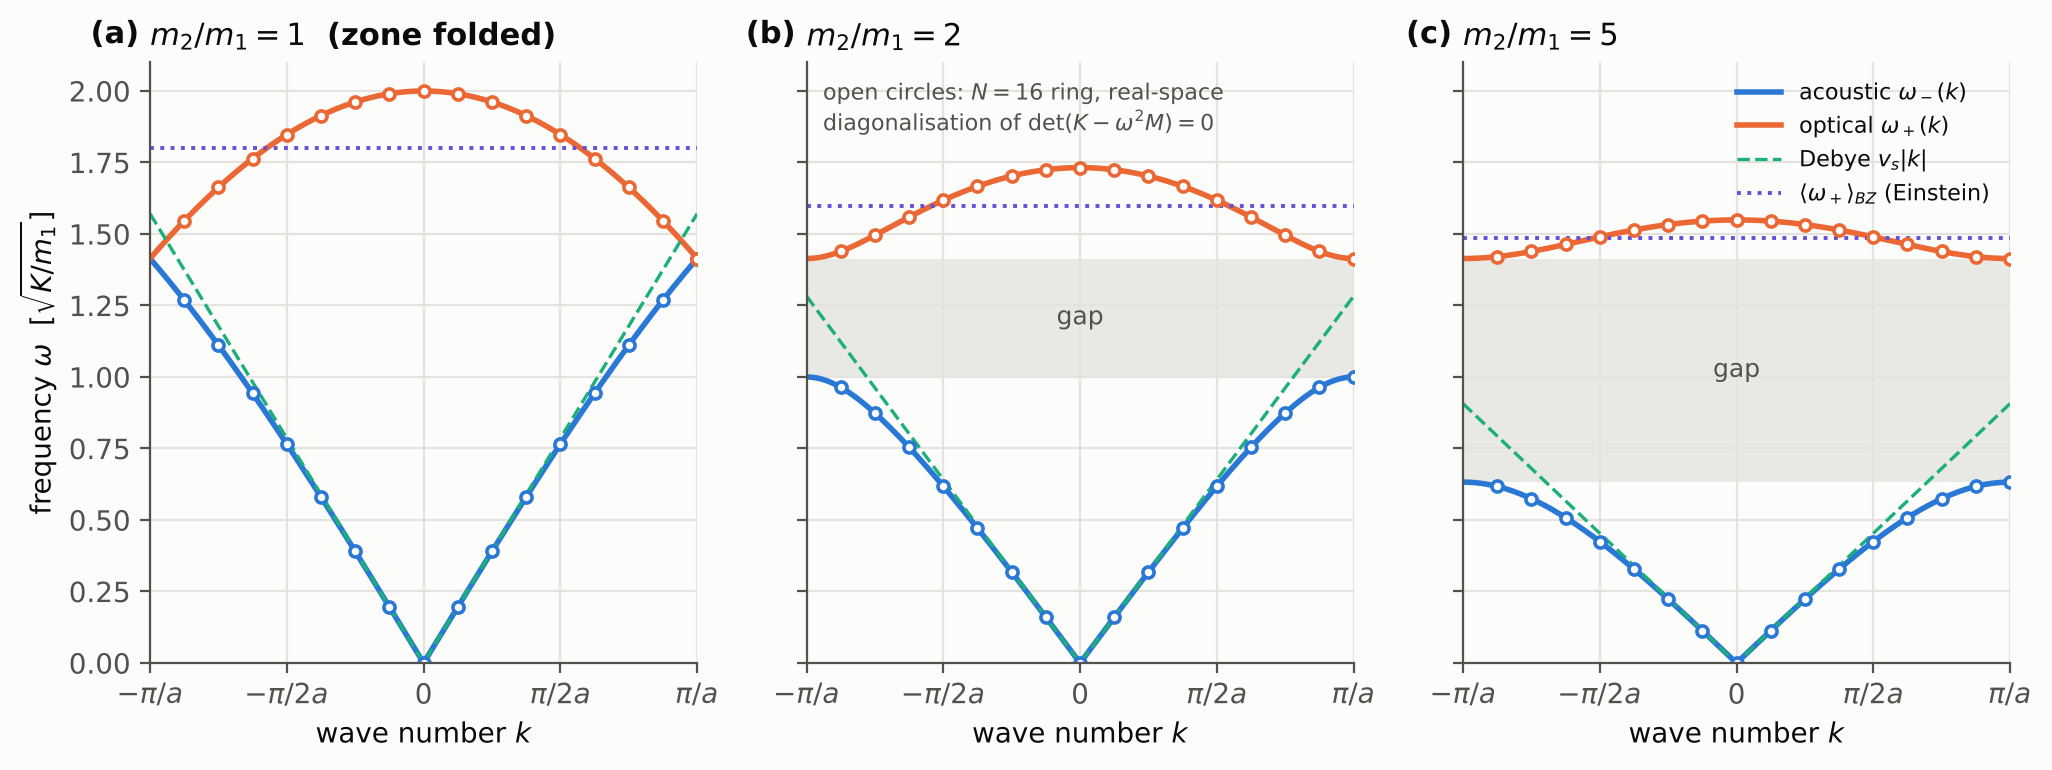
\includegraphics[width=\textwidth]{dispersion.png}
\caption{Ramas acústica (azul) y óptica (naranja) para tres cocientes de masas
con $K_1=K_2$. Los círculos son las $2N$ frecuencias de un anillo de $N=16$
celdas obtenidas diagonalizando directamente $\det(K-\omega^2M)=0$ en el
espacio real, sin usar el teorema de Bloch: coinciden con las curvas en los $N$
valores de $k$ permitidos por Born–von Kármán (diferencia máxima
$\sim2\times10^{-8}$, error de redondeo del modo de traslación). En verde,
la recta de Debye $\vs|k|$; en violeta, el nivel de Einstein
$\avg{\omega_+}_{\rm BZ}$. (a) Con masas iguales el gap se cierra: es la
cadena monoatómica de parámetro $a/2$ con su zona «plegada».}
\label{fig:dispersion}
\end{figure}

\subsection{Vectores propios: qué se mueve en cada rama}

De la primera fila de $(D-\omega^2)\bm e=0$, el cociente de amplitudes físicas
es
\begin{equation}
\frac{u_2}{u_1}=\frac{\sigma-m_1\omega^2}{K_1+K_2\ee^{-\ii ka}} .
\end{equation}
\begin{itemize}
\item En $k=0$, rama acústica: $u_2/u_1=1$; la celda se traslada rígidamente.
\item En $k=0$, rama óptica: $u_2/u_1=-m_1/m_2$; los átomos oscilan en
  contrafase y el \textbf{centro de masas de cada celda permanece en reposo}.
\item En $k=\pi/a$ (con $K_1=K_2$, $m_2>m_1$): en la rama acústica solo se
  mueven los átomos pesados y en la óptica solo los ligeros; cada subred vibra
  como si la otra fuera una pared rígida, de ahí las frecuencias
  $\sqrt{2K/m}$.
\end{itemize}
La Fig.~\ref{fig:eigen} muestra el cociente (medido desde la posición de cada
átomo, que con $K_1=K_2$ lo hace real:
$\frac{2K-m_1\omega^2}{2K\cos(ka/2)}$) y las configuraciones en el espacio real.

\begin{figure}[t]
\centering
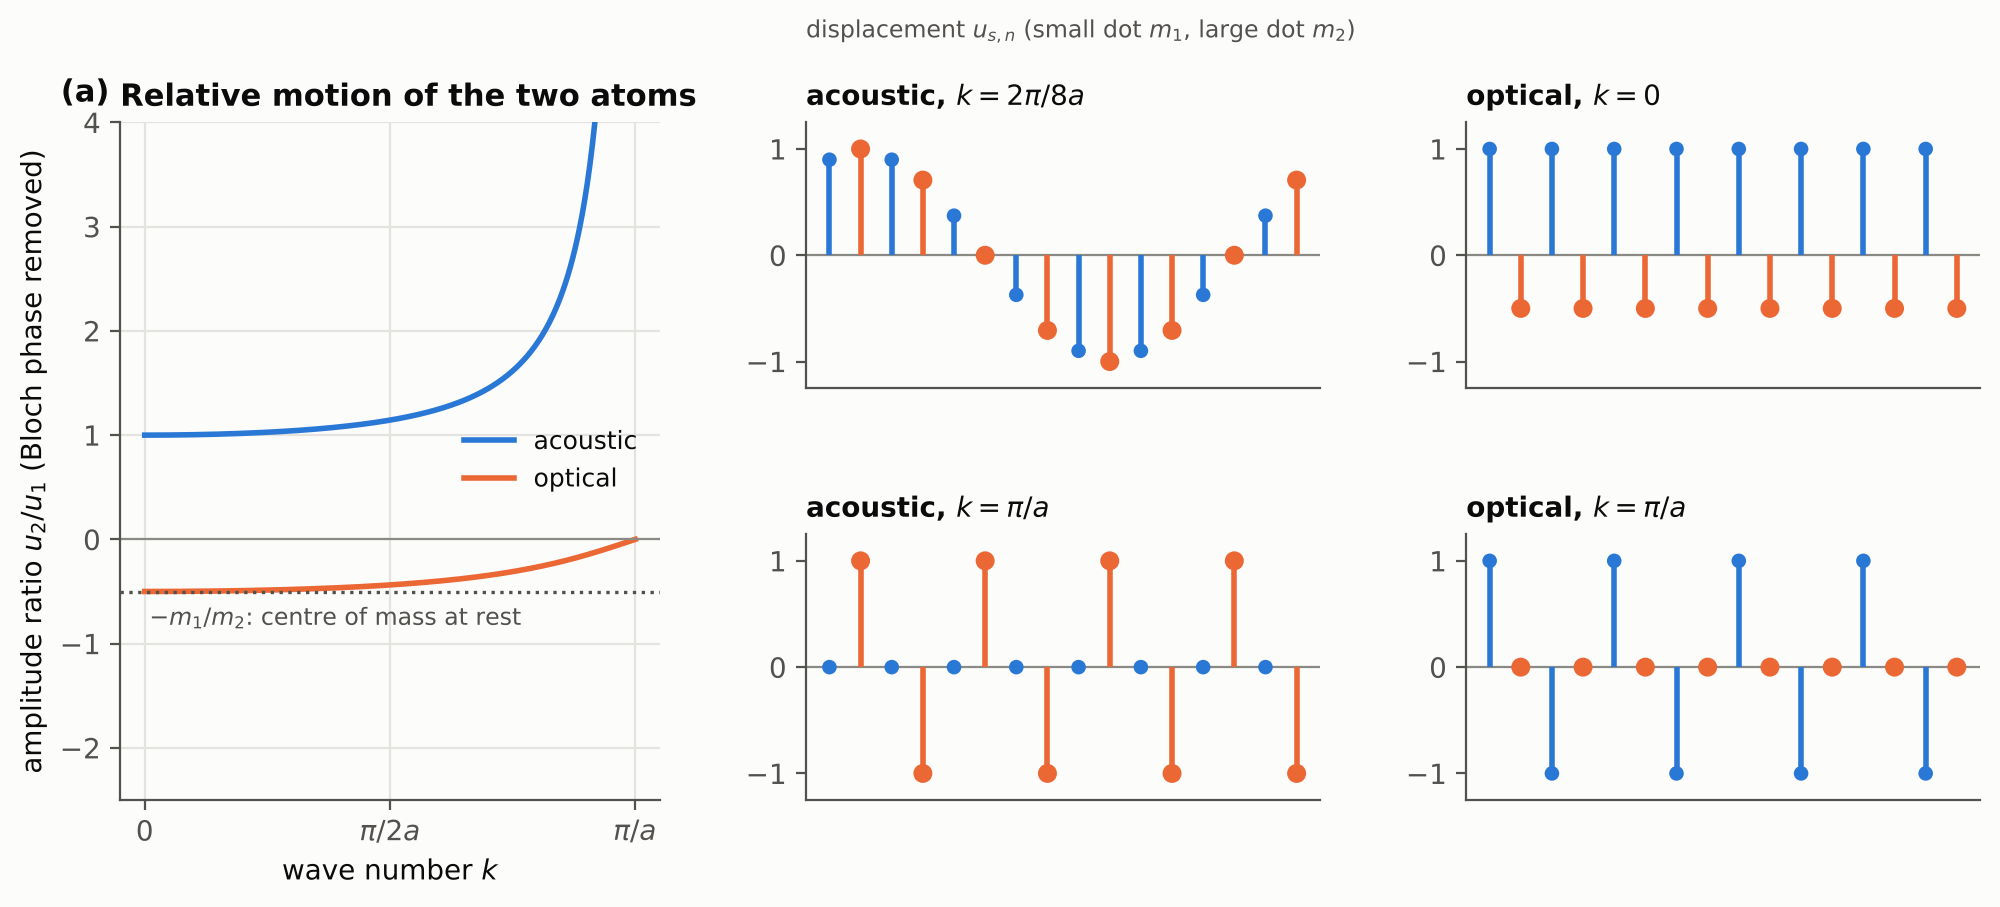
\includegraphics[width=\textwidth]{eigenvectors.png}
\caption{(a) Cociente de amplitudes $u_2/u_1$ a lo largo de la zona de
Brillouin ($m_2/m_1=2$): positivo (en fase) en la rama acústica, negativo
(contrafase) en la óptica, con el valor $-m_1/m_2$ en $k=0$. (b)–(e)
Desplazamientos de los $16$ átomos de un anillo de $8$ celdas para cuatro modos
representativos.}
\label{fig:eigen}
\end{figure}

\subsection{Casos límite y generalización}

\paragraph{Masas iguales, $m_1=m_2$, $K_1=K_2$.} El gap se cierra y las dos
ramas son la dispersión de la cadena monoatómica de parámetro $a'=a/2$,
$\omega=2\sqrt{K/m}\,|\sin(qa'/2)|$, «plegada» sobre la zona de Brillouin más
pequeña de la celda doble. Elegir una celda doble es una decisión del
\Eobs{}, no del \Eesc: la física no cambia.

\paragraph{Contraste de masas grande, $m_2\gg m_1$.} La rama óptica se vuelve
casi plana, $\omega_+\simeq\sqrt{2K/m_1}$: los átomos ligeros vibran casi
independientemente en la «jaula» de los pesados. Es exactamente la hipótesis de
Einstein, que pasa a ser casi exacta para esa rama. La rama acústica tiende a
la de una cadena monoatómica de átomos pesados.

\paragraph{Contraste de rigideces, $K_1\neq K_2$.} Incluso con masas iguales se
abre un gap (Fig.~\ref{fig:gapmap}b): basta con que la celda real contenga dos
átomos no equivalentes. Es la versión fonónica de una cadena dimerizada.

\begin{figure}[t]
\centering
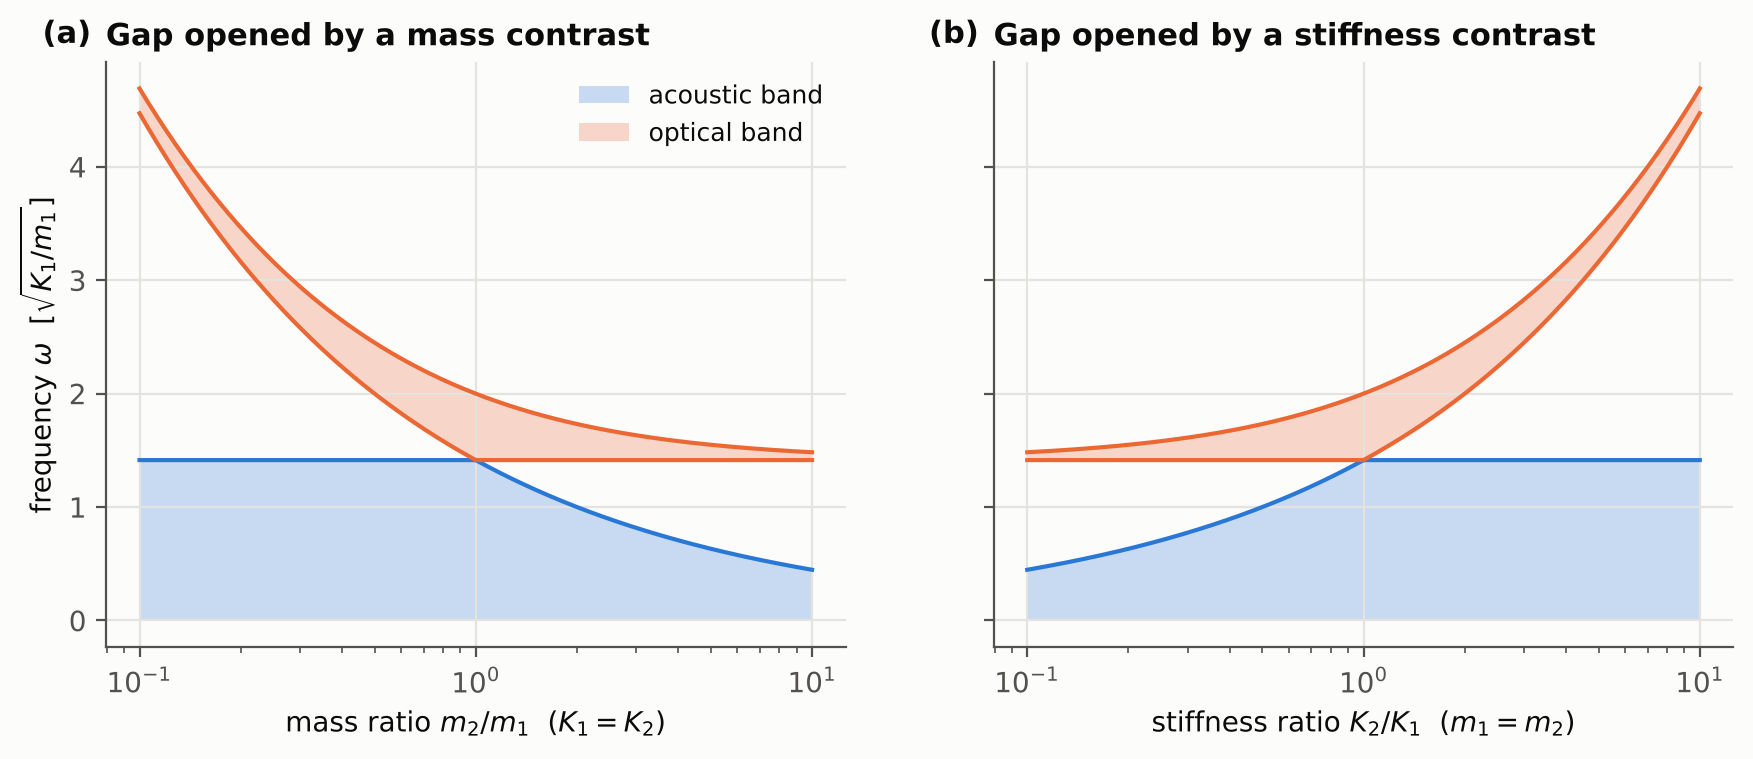
\includegraphics[width=0.92\textwidth]{gap_map.png}
\caption{Bandas permitidas en función de (a) el cociente de masas con $K_1=K_2$ y
(b) el cociente de rigideces con $m_1=m_2$. En ambos casos el gap solo se
cierra cuando los dos átomos de la celda son equivalentes.}
\label{fig:gapmap}
\end{figure}

% =====================================================================
\section{Densidad de estados de la cadena diatómica}

\subsection{Expresión cerrada}

Invertimos la ecuación secular para expresar $s\equiv\sin^2(ka/2)$ en función
de $\omega$. De $\det(D-\omega^2)=0$,
$(\sigma/m_1-\omega^2)(\sigma/m_2-\omega^2)=|D_{12}|^2$, y desarrollando el
producto el término $\sigma^2$ se cancela exactamente:
\begin{equation}
s(\omega)=\frac{m_1m_2\,\omega^2\left(\sigma/\mu-\omega^2\right)}{4K_1K_2}.
\end{equation}
Como $ka=2\arcsin\sqrt{s}$, $\dd k/\dd\omega=\frac{1}{a}\frac{s'(\omega)}{\sqrt{s(1-s)}}$
y, contando $\pm k$,
\begin{equation}
\boxed{\;g(\omega)=\frac{1}{\pi}\,\frac{|s'(\omega)|}{\sqrt{s(1-s)}}\,,
\qquad s'(\omega)=\frac{m_1m_2\,\omega\,(\sigma/\mu-2\omega^2)}{2K_1K_2}\,,
\qquad 0<s(\omega)<1\;}
\end{equation}
y $g=0$ fuera de las bandas. Comprobaciones inmediatas:
\begin{itemize}
\item $\omega\to0$: $g(0)=\frac{a}{\pi\vs}$, la DOS plana de un medio elástico
  (es la que usa Debye).
\item En los cuatro bordes de banda ($s=1$, o bien $s'=0$ en el techo óptico)
  $g$ diverge como $(\omega_c-\omega)^{-1/2}$: singularidades de van Hove.
\item El número acumulado de modos también es cerrado:
\begin{equation}
N(\omega)=\begin{cases}
\frac2\pi\arcsin\sqrt{s(\omega)} & \text{banda acústica}\\
1 & \text{gap}\\
2-\frac2\pi\arcsin\sqrt{s(\omega)} & \text{banda óptica}
\end{cases}
\end{equation}
(la rama óptica \emph{decrece} con $|k|$), con $N(\infty)=2$: un modo acústico
y uno óptico por celda.
\end{itemize}

\begin{codigo}
La DOS se calcula por tres vías independientes en \code{dos.py}: la fórmula
cerrada (\code{analytic\_dos}), el histograma de las frecuencias sobre una malla
fina de $k$ (\code{sampled\_dos}) y el histograma de los $2N$ autovalores de un
anillo finito diagonalizado en el espacio real (\code{histogram\_dos}). Como
$N(\omega)$ es exacta, el promedio exacto de $g$ en cada intervalo del
histograma es $\Delta N/\Delta\omega$ (\code{bin\_averaged\_dos}): la
diferencia máxima con el muestreo de $2\times10^5$ valores de $k$ es
$3\times10^{-4}$ y las tres vías están normalizadas a $2$ hasta el redondeo.
\end{codigo}

\begin{figure}[t]
\centering
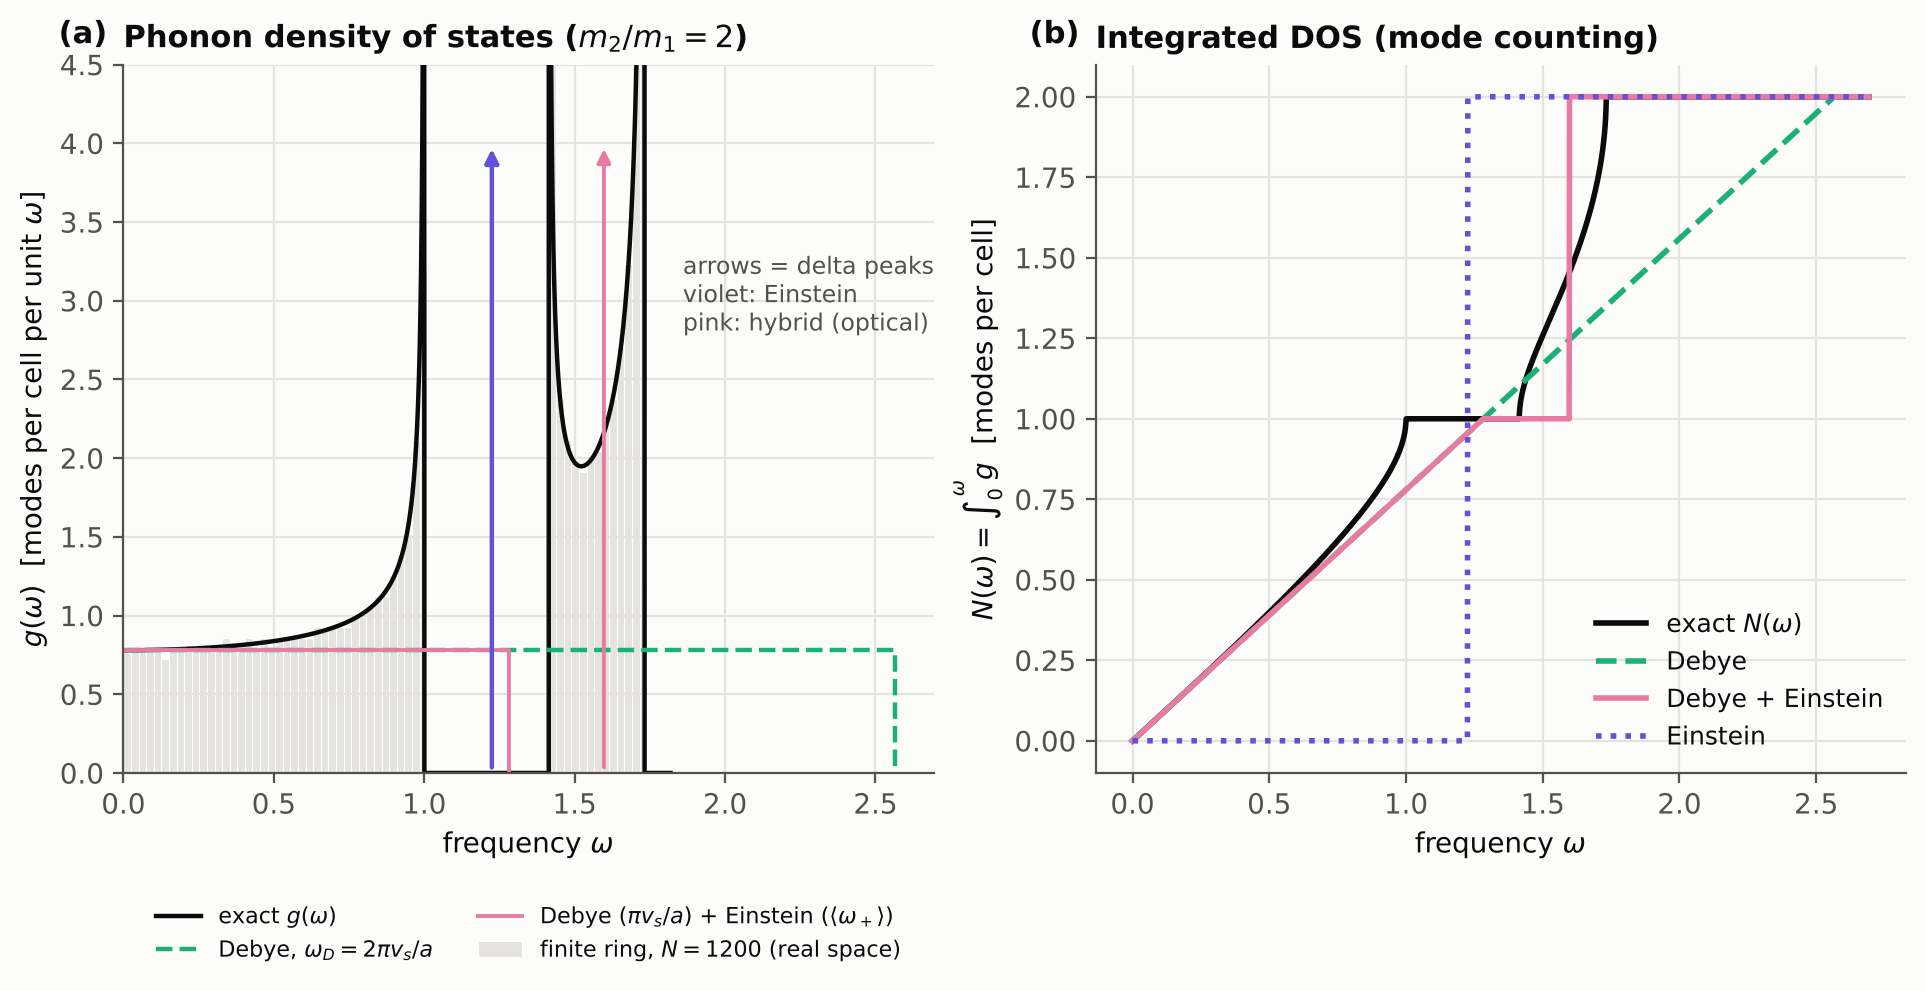
\includegraphics[width=\textwidth]{dos.png}
\caption{(a) DOS exacta (negro) frente al histograma de un anillo de $1200$
celdas (gris), la DOS plana de Debye (verde), la del modelo híbrido (rosa:
Debye para la rama acústica hasta $\pi\vs/a$ más un pico de Einstein en
$\avg{\omega_+}$) y el pico de Einstein (violeta). (b) Número acumulado de
modos: Debye reparte los dos modos por celda uniformemente hasta
$2\pi\vs/a=2.57$, muy por encima del techo real $1.73$.}
\label{fig:dos}
\end{figure}

\subsection{Lectura física de la Fig.~\ref{fig:dos}}

La DOS exacta tiene tres rasgos que ningún modelo sencillo reproduce a la vez:
la meseta acústica a baja frecuencia (que Debye sí captura), la acumulación de
modos en los bordes de banda (van Hove) y el gap. Debye coloca modos donde no
los hay (entre $1.73$ y $2.57$) para compensar el número total; Einstein coloca
todos los modos en una sola frecuencia. Como $C_V$ es un promedio de $g$
ponderado por $c(\hbar\omega/\kB T)$, que es una función suave, los
detalles finos de $g$ se lavan: la pregunta cuantitativa es \emph{cuánto}.

% =====================================================================
\section{Calor específico: resultado numérico frente a los modelos}

\subsection{Cálculo numérico}

En lugar de integrar \eqref{eq:dosint} en $\omega$, donde $g$ tiene
singularidades, integramos en $k$, donde todo es suave:
\begin{equation}
\frac{C_V}{N\kB}=\frac{a}{\pi}\int_0^{\pi/a}\dd k\,\sum_{b=\pm}c\!\left(\frac{\hbar\omega_b(k)}{\kB T}\right),
\end{equation}
con cuadratura de Gauss–Legendre (convergencia exponencial). A baja
temperatura el integrando acústico solo es apreciable en $k\lesssim 40\kB
T/\hbar\vs$, así que el intervalo se parte ahí para concentrar nodos donde vive
la función. El resultado coincide con la integral sobre la DOS analítica
(\code{scipy.integrate.quad}) hasta $10^{-12}$ y con la suma exacta sobre los
modos de un anillo de $400$ celdas hasta $10^{-4}$ (efecto de tamaño finito).

\subsection{Resultados}

\begin{figure}[t]
\centering
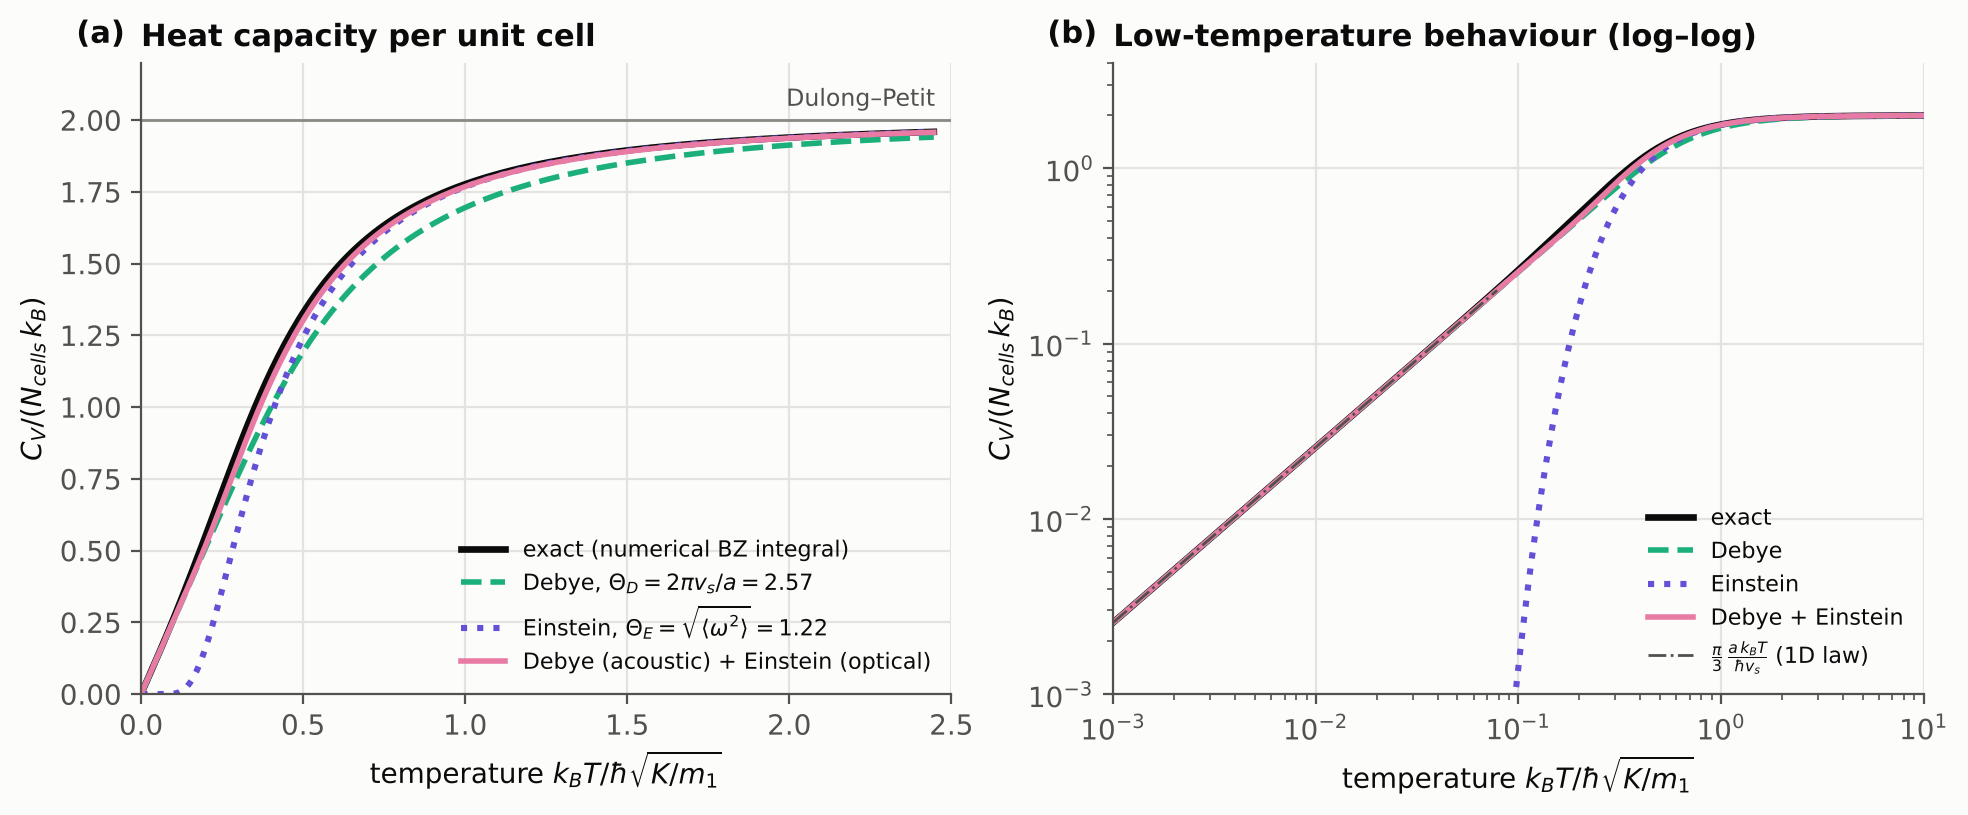
\includegraphics[width=\textwidth]{heat_capacity.png}
\caption{Calor específico por celda de la cadena de referencia ($m_2/m_1=2$).
(a) Escala lineal: el exacto (negro) frente a Debye con $\Theta_D=2\pi\vs/a$,
Einstein con $\Theta_E=\sqrt{\avg{\omega^2}}$ y el híbrido. (b) Escala
log–log: a baja $T$ el exacto sigue la ley lineal \eqref{eq:lowT} (pendiente
numérica $2.56510$ frente a la teórica $\pi a/3\vs=2.56510$) y Einstein cae
exponencialmente.}
\label{fig:cv}
\end{figure}

\begin{table}[h]
\centering
\small
\begin{tabular}{@{}ccccc@{}}
\toprule
$\kB T$ & exacto & Debye & Einstein & Debye + Einstein\\
\midrule
0.01 & 0.02566 & 0.02565 & $2\times10^{-49}$ & 0.02565\\
0.1  & 0.2629  & 0.2565  & 0.00144 & 0.2565\\
0.3  & 0.8553  & 0.7654  & 0.5816  & 0.8141\\
0.5  & 1.3286  & 1.1931  & 1.2411  & 1.3023\\
1.0  & 1.7764  & 1.6952  & 1.7677  & 1.7684\\
2.0  & 1.9393  & 1.9129  & 1.9387  & 1.9372\\
\bottomrule
\end{tabular}
\caption{$C_V/N\kB$ de la cadena de referencia. Los modelos usan los
parámetros fijados por la física (no ajustados): $\Theta_D=2\pi\hbar\vs/a\kB=2.565$,
$\Theta_E=\sqrt{\avg{\omega^2}}=1.225$ y, en el híbrido,
$\omega_D^{\rm ac}=\pi\vs/a=1.283$ y $\omega_E=\avg{\omega_+}_{\rm BZ}=1.597$.}
\label{tab:cv}
\end{table}

Las conclusiones cuantitativas para $m_2/m_1=2$ son:
\begin{enumerate}
\item \textbf{Bajas temperaturas.} Debye (y por tanto el híbrido) es exacto; el
  error relativo es $2\times10^{-4}$ en $\kB T=10^{-2}$ y $2\times10^{-6}$ en
  $\kB T=10^{-3}$. Einstein falla por
  completo (49 órdenes de magnitud en $\kB T=0.01$).
\item \textbf{Altas temperaturas.} Los tres tienden a Dulong–Petit. Einstein con
  $\omega_E^2=\avg{\omega^2}$ reproduce por construcción la corrección
  $1/T^2$ (en $\kB T=10$: exacto $1.997503$, desarrollo $1.997500$) y es el
  mejor de los tres por encima de $\kB T\approx1$.
\item \textbf{Región intermedia} ($\kB T\sim0.1$–$0.5$, donde $C_V$ crece
  más deprisa). Aquí está la física de la DOS real: Debye subestima $C_V$
  hasta un $11\%$ porque reparte modos hasta $2.57$, donde todavía están
  congelados; el híbrido reduce el error máximo al $6\%$.
\item \textbf{Ajustes.} Ajustando por mínimos cuadrados un único $\Theta$ en
  $\kB T\in[0.02,3]$: Debye da $\Theta_D=2.256$ con error cuadrático medio
  $0.020$, pero entonces deja de ser exacto a bajas $T$ (error relativo máximo
  $14\%$); Einstein da $\Theta_E=0.962$ con error cuadrático $0.14$ y sigue
  fallando cualitativamente a bajas $T$. Un buen ajuste global no implica una
  buena física: el parámetro ajustado esconde la estructura de $g(\omega)$.
\end{enumerate}

\subsection{Descomposición por ramas}

\begin{figure}[t]
\centering
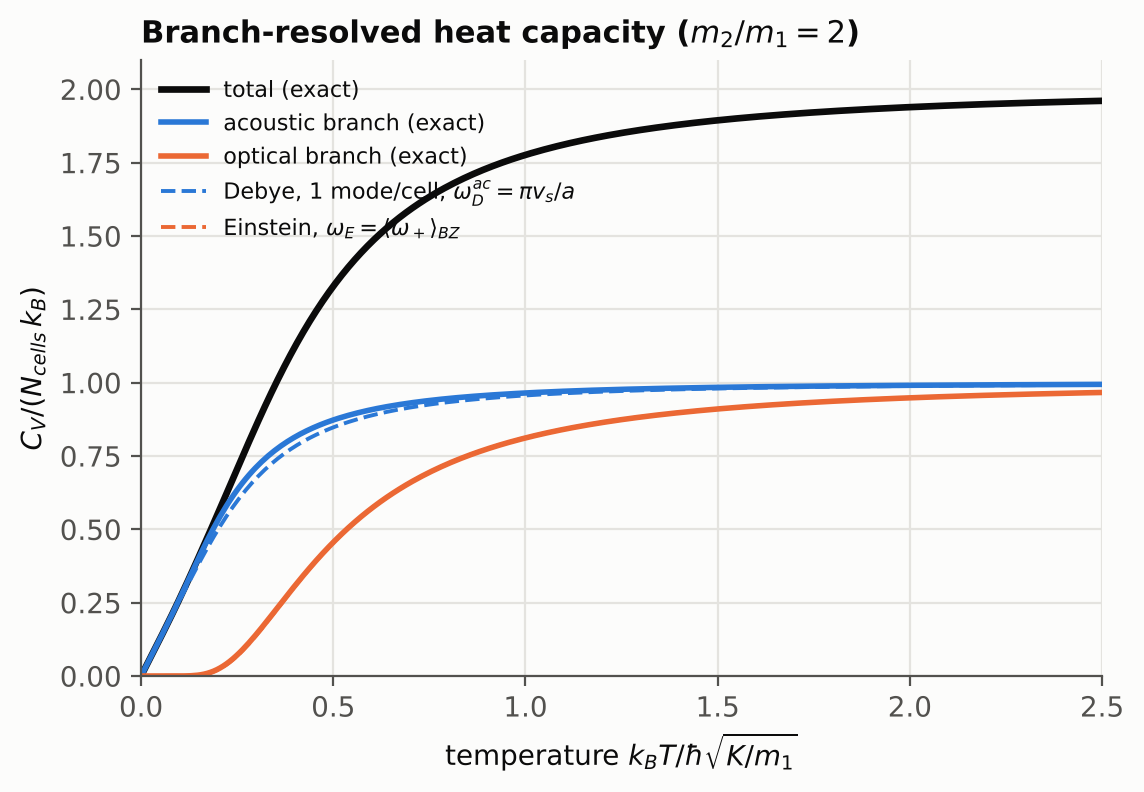
\includegraphics[width=0.62\textwidth]{heat_capacity_branches.png}
\caption{Contribuciones acústica y óptica al calor específico (cada una satura
en $\kB$ por celda) y los modelos de Debye (1 modo/celda) y Einstein aplicados
a cada rama por separado.}
\label{fig:branches}
\end{figure}

Como el sistema es ideal, $C_V=C_{\rm ac}+C_{\rm op}$ exactamente
(Fig.~\ref{fig:branches}). La rama óptica está congelada por debajo de
$\kB T\approx0.1$ (aporta el $0.02\%$ de $C_V$ en $\kB T=0.1$), el $10\%$ en
$\kB T=0.25$ y el $34\%$ en $\kB T=0.5$. Toda la física de bajas temperaturas
es acústica, y esto justifica el modelo híbrido: Debye donde la dispersión es
lineal, Einstein donde la rama es estrecha. En la figura se ve además dónde
reside el error del híbrido: en la parte acústica, porque la rama real se curva
(y acumula modos en su techo) mientras que Debye la mantiene lineal.

\subsection{Dependencia con el cociente de masas}

\begin{figure}[t]
\centering
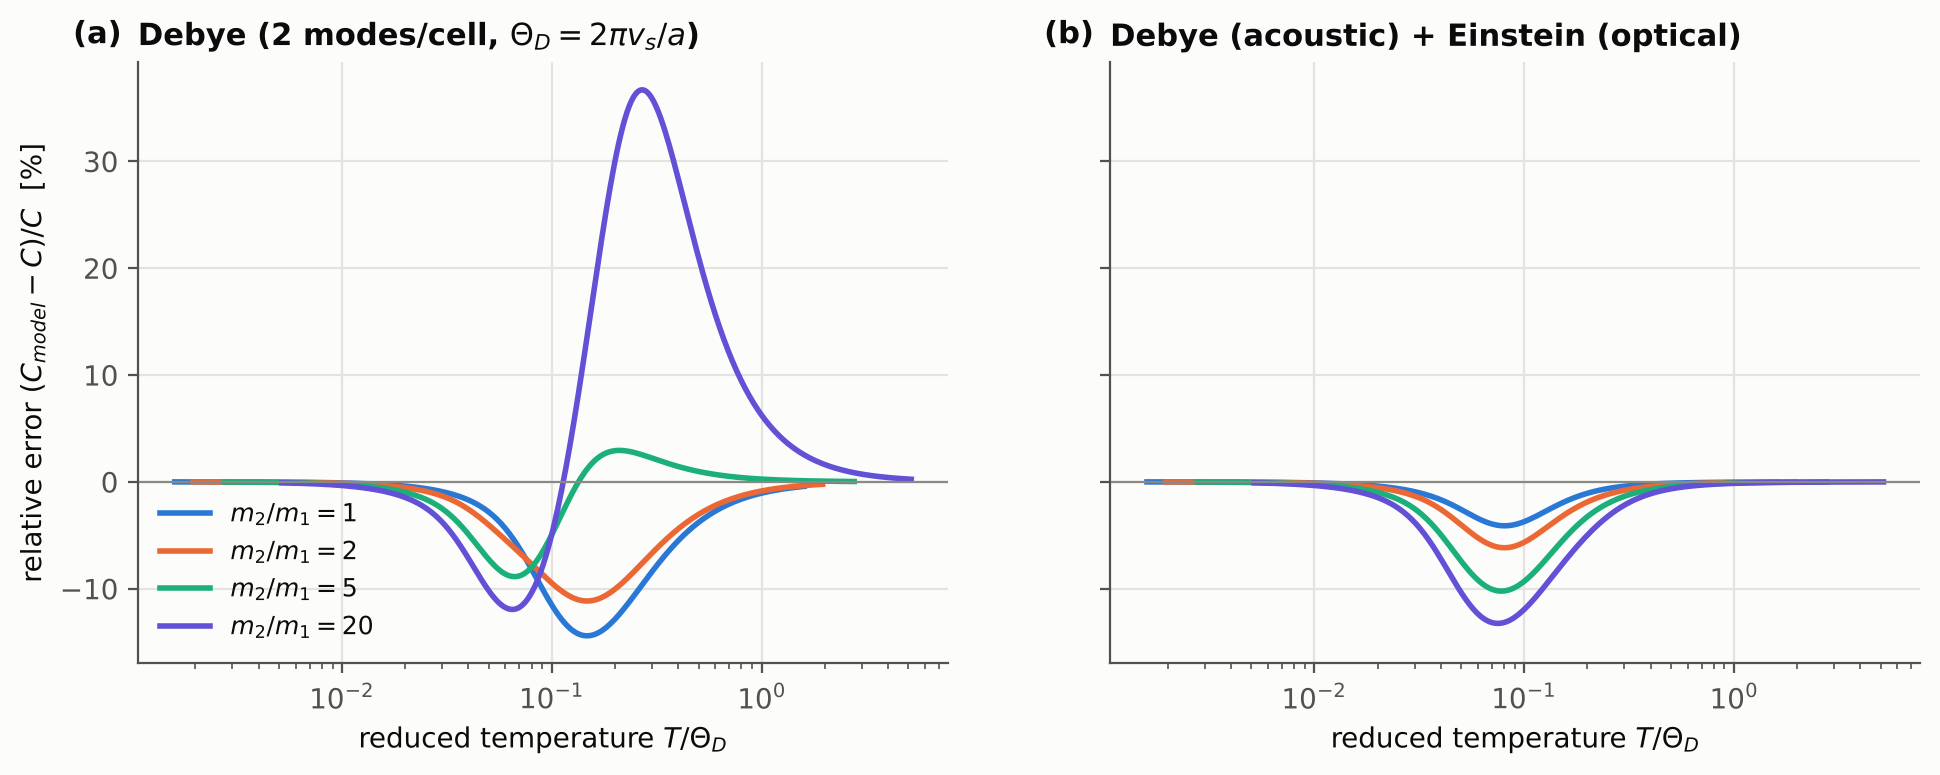
\includegraphics[width=\textwidth]{model_errors.png}
\caption{Error relativo de (a) Debye y (b) el modelo híbrido frente a $T/\Theta_D$
para varios cocientes de masas.}
\label{fig:errors}
\end{figure}

La Fig.~\ref{fig:errors} resume cómo cambia la calidad de los modelos con
$m_2/m_1$:
\begin{center}
\small
\begin{tabular}{@{}ccc@{}}
\toprule
$m_2/m_1$ & error máx.\ Debye & error máx.\ Debye + Einstein\\
\midrule
1  & $14.4\%$ & $4.1\%$\\
2  & $11.2\%$ & $6.2\%$\\
5  & $8.9\%$  & $10.2\%$\\
20 & $36.7\%$ & $13.2\%$\\
\bottomrule
\end{tabular}
\end{center}
\begin{itemize}
\item \textbf{Debye} empeora drásticamente para contrastes grandes: cuanto más
  pesado es el segundo átomo, menor es $\vs$, menor $\Theta_D$ y peor describe
  la rama óptica, que está a una frecuencia $\sqrt{2K/m_1}$ que no depende de
  $m_2$. Para $m_2/m_1=20$ sobrestima $C_V$ un $37\%$ (pone a vibrar modos
  ópticos que en realidad están congelados).
\item \textbf{El híbrido} sigue una tendencia aparentemente paradójica: su error
  \emph{crece} con $m_2/m_1$ aunque la rama óptica sea cada vez más plana
  (Einstein cada vez más exacto). La razón es que el error residual es el de
  Debye aplicado a la rama acústica, que con contraste grande es la de una
  cadena monoatómica de átomos pesados, sinusoidal y con una gran singularidad
  de van Hove en su techo; su error de Debye es $\simeq14\%$, el mismo que el
  de la cadena monoatómica de la primera fila. Para $m_2/m_1=1$ el híbrido es
  muy bueno porque la «rama óptica» es la parte superior plegada de la misma
  sinusoide y $\avg{\omega_+}$ la representa bien.
\end{itemize}

\subsection{Temperatura de Debye efectiva}

\begin{figure}[t]
\centering
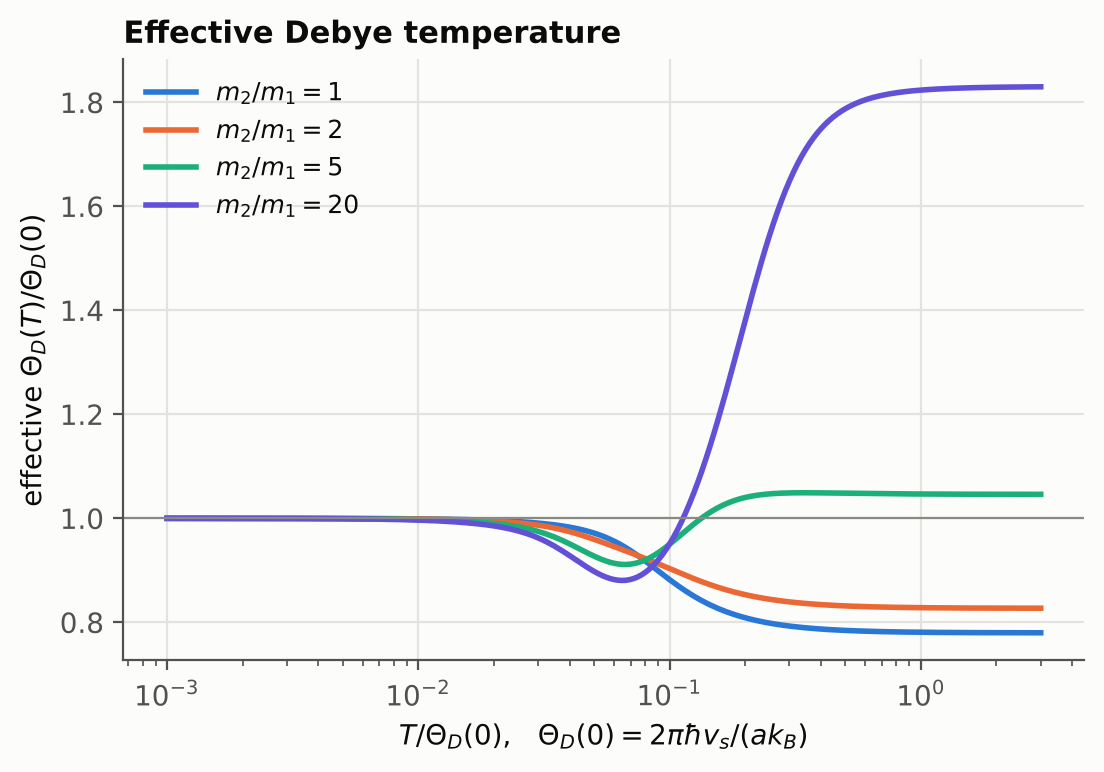
\includegraphics[width=0.62\textwidth]{debye_temperature.png}
\caption{Temperatura de Debye efectiva $\Theta_D(T)$, normalizada a su valor a
$T=0$, para varios cocientes de masas.}
\label{fig:thetaD}
\end{figure}

La Fig.~\ref{fig:thetaD} muestra $\Theta_D(T)/\Theta_D(0)$. Todas las curvas
parten de $1$ (Debye exacto a $T\to0$) y bajan en cuanto se excitan los modos
acústicos próximos al techo de la banda: la DOS real los acumula por debajo del
corte de Debye (van Hove) y el cristal se «ablanda». Para $m_2/m_1=1$ y $2$ el
descenso es monótono; para $m_2/m_1=5$ y $20$ hay un mínimo hacia
$T\approx0.06\,\Theta_D(0)$ seguido de una subida, cuando se descongela la rama
óptica. A alta temperatura todas saturan en
$\sqrt{3\avg{\omega^2}}/\Theta_D(0)$: $0.78$, $0.83$, $1.05$ y $1.83$ para
$m_2/m_1=1,2,5,20$. Para contrastes grandes la saturación supera
$1$: la rama óptica, de alta frecuencia y con la mitad de los modos, «endurece»
el cristal frente a lo que predice la velocidad del sonido. Es exactamente lo
que se observa experimentalmente en sólidos con bases de masas muy distintas, y
la razón por la que una única temperatura de Debye tabulada nunca describe
bien todo el rango de temperaturas.

% =====================================================================
\section{Otros observables}

\subsection{Energía interna, entropía y energía libre}

\begin{figure}[t]
\centering
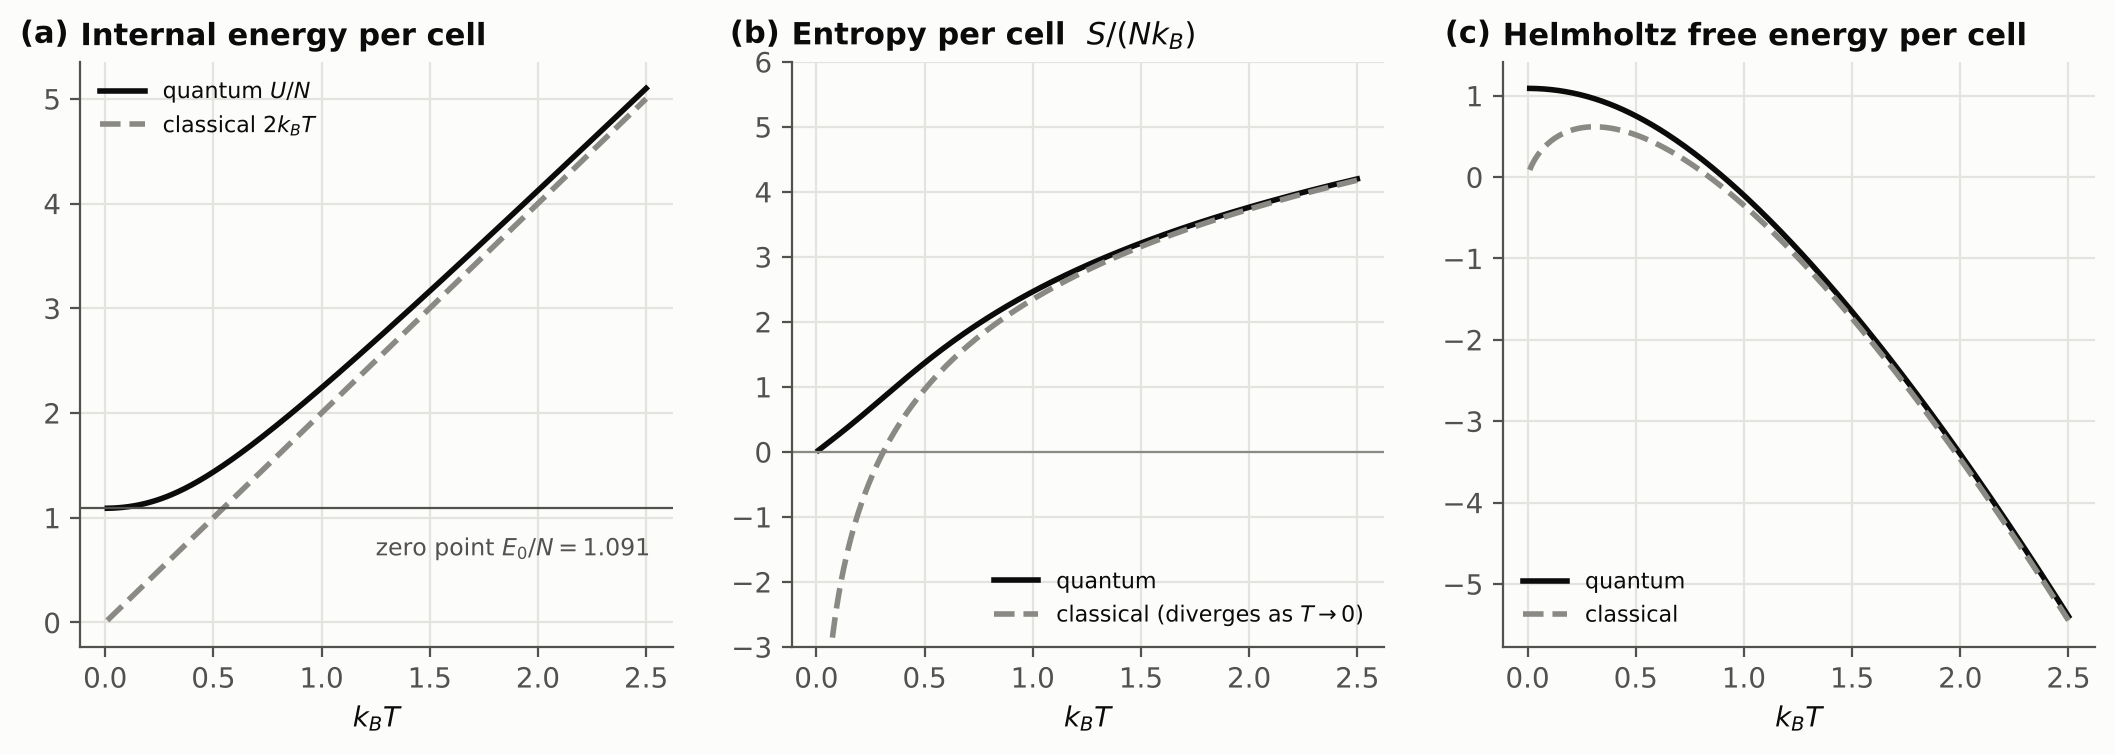
\includegraphics[width=\textwidth]{thermo_functions.png}
\caption{(a) Energía interna por celda: a $T=0$ queda la energía de punto cero
$E_0/N=1.091$; a alta $T$ la curva cuántica tiende a la clásica $2\kB T$ (no
a $2\kB T+E_0/N$: el punto cero se cancela en el desarrollo
$\frac{\hbar\omega}{2}\coth\frac{y}{2}=\kB T+\frac{\hbar^2\omega^2}{12\kB T}+\dots$).
(b) Entropía: la cuántica se anula a $T=0$ (tercer principio); la clásica
diverge a $-\infty$, señal de que la contabilidad clásica de microestados falla
a bajas temperaturas. (c) Energía libre de Helmholtz.}
\label{fig:thermo}
\end{figure}

La Fig.~\ref{fig:thermo} muestra $U$, $S$ y $F$ por celda en el tratamiento
cuántico y clásico. Dos comentarios de mecánica estadística:
(i) la entropía clásica negativa a bajas $T$ es el mismo síntoma que la
entropía negativa de Sackur–Tetrode a bajas temperaturas: discretizar el
espacio fásico en celdas de volumen $h$ deja de tener sentido cuando la acción
típica es del orden de $\hbar$; (ii) la consistencia termodinámica
$S=-\partial F/\partial T$, $C_V=\partial U/\partial T$, $U=F+TS$ se comprueba
numéricamente en los tests hasta $10^{-6}$.

\subsection{Fluctuaciones de los desplazamientos: no hay orden de largo alcance en 1D}

Este es el observable más interesante físicamente. Expandiendo en modos
normales, $u_{s,n}=N^{-1/2}\sum_{k,b}(e_s/\sqrt{m_s})\ee^{\ii kna}Q_{k,b}$, y
usando que cada coordenada normal es un oscilador de masa unidad con
\begin{equation}
\avg{|Q_{k,b}|^2}=\frac{\hbar}{2\omega}\coth\frac{\hbar\omega}{2\kB T}
\ \xrightarrow{\ \hbar\to0\ }\ \frac{\kB T}{\omega^2},
\end{equation}
calculamos el \textbf{desplazamiento relativo cuadrático medio} de dos átomos
separados $r$ celdas,
\begin{equation}
G_{ss'}(r)=\avg{(u_{s',n+r}-u_{s,n})^2}
=\frac{a}{2\pi}\int_{\rm BZ}\dd k\sum_b\avg{|Q_{k,b}|^2}
\left|\frac{e_{s'}\ee^{\ii kra}}{\sqrt{m_{s'}}}-\frac{e_s}{\sqrt{m_s}}\right|^2 .
\end{equation}
El factor $|\cdots|^2\propto k^2$ para la rama acústica cuando $k\to0$ hace
que $G(r)$ sea finita para cada $r$, pero su comportamiento con $r$ es muy
revelador (Fig.~\ref{fig:disp}a):
\begin{itemize}
\item \textbf{Clásicamente} el resultado es exacto y sencillo:
  $G_{11}(r)=r\,\kB T\left(\frac{1}{K_1}+\frac{1}{K_2}\right)$. Los
  estiramientos de los enlaces son variables gaussianas independientes de
  varianza $\kB T/K_i$ (equipartición aplicada a cada muelle), y la separación
  entre dos átomos es la suma de $2r$ de ellos: un paseo aleatorio. El código
  lo reproduce con error relativo $<10^{-8}$.
\item \textbf{Cuánticamente a $T=0$}, $G(r)\simeq\frac{\hbar a}{\pi M\vs}\ln r$:
  crecimiento logarítmico (pendiente numérica $0.259899$ frente a la teórica
  $0.259899$).
\end{itemize}
Como $G(r)\to\infty$ cuando $r\to\infty$, las posiciones de átomos lejanos no
están correlacionadas: \textbf{una cadena 1D no tiene orden posicional de largo
alcance} a ninguna temperatura (argumento de Landau–Peierls). Es la misma
moraleja que la ausencia de transición de fase en el modelo de Ising 1D: en
una dimensión las fluctuaciones de longitud de onda larga ganan siempre.
Equivalentemente, el desplazamiento cuadrático medio de un átomo en un anillo
de $N$ celdas (eliminando la traslación rígida) diverge con $N$
(Fig.~\ref{fig:disp}b): $\avg{u_1^2}=\frac{N}{12}\kB T\left(\frac1{K_1}+\frac1{K_2}\right)$
clásicamente (verificado: $0.166667\,N\kB T$ con nuestros parámetros) y
$\simeq\frac{\hbar a}{2\pi M\vs}\ln N$ a $T=0$. El factor de Debye–Waller
$\ee^{-q^2\avg{u^2}}$ se anula en el límite termodinámico: un cristal 1D no
daría picos de Bragg nítidos.

\begin{figure}[t]
\centering
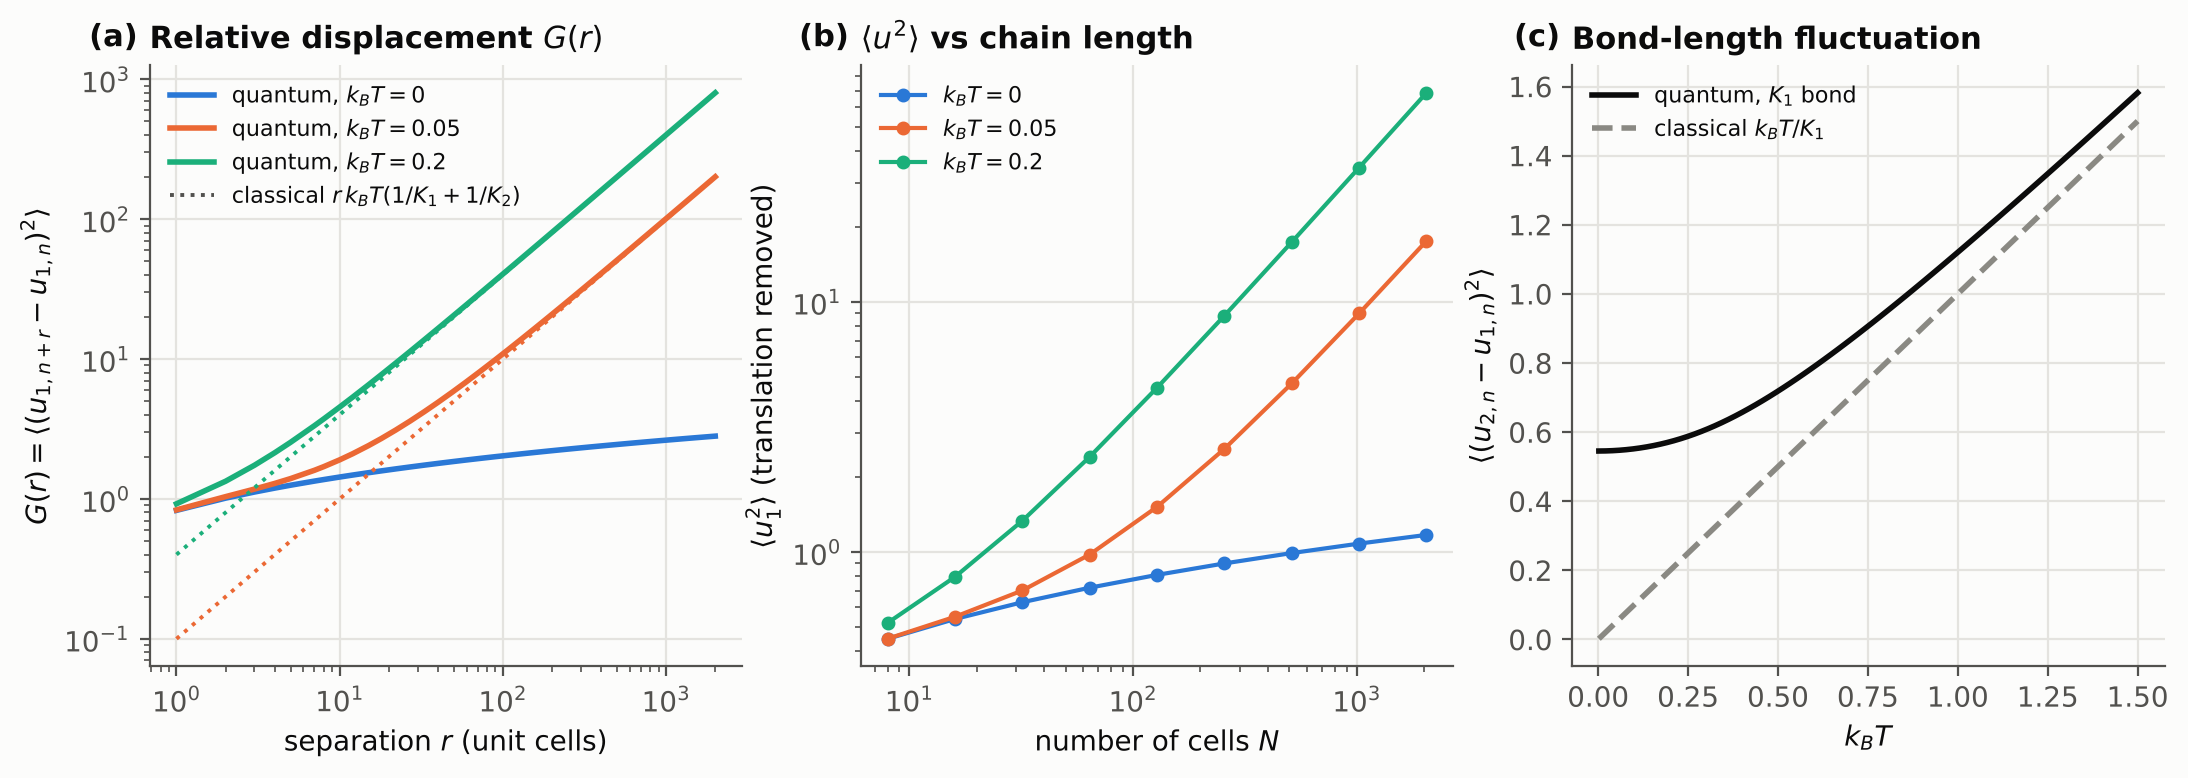
\includegraphics[width=\textwidth]{displacements.png}
\caption{(a) Desplazamiento relativo $G(r)$ cuántico para tres temperaturas
(continuo) y el resultado clásico $r\kB T(1/K_1+1/K_2)$ (punteado): a
distancias cortas domina el punto cero, a distancias largas el crecimiento
lineal térmico. (b) $\avg{u_1^2}$ en anillos de $N$ celdas: lineal en $N$ a
$T>0$, logarítmico a $T=0$. (c) Fluctuación de un enlace: el punto cero
($0.545$ a $T=0$) frente a la recta clásica $\kB T/K_1$.}
\label{fig:disp}
\end{figure}

\subsection{Fluctuación de enlace}

Las fluctuaciones \emph{locales} sí están bien definidas: la fluctuación del
enlace $K_1$, $\avg{(u_{2,n}-u_{1,n})^2}$, es finita a toda temperatura
(Fig.~\ref{fig:disp}c). A $T=0$ vale $0.545$ (en unidades
$\hbar/\sqrt{Km_1}$) por el movimiento de punto cero, y a alta $T$ tiende a la
equipartición $\kB T/K_1$. Es la magnitud que entra en un criterio de tipo
Lindemann para la fusión, y muestra de nuevo la transición entre régimen
cuántico (meseta) y clásico (recta).

% =====================================================================
\section{Validación independiente: dinámica de Langevin}\label{sec:langevin}

\subsection{Motivación}

Todo lo anterior usa modos normales. Para comprobar la física por un camino
completamente distinto simulamos la dinámica \emph{clásica} de un anillo de
átomos acoplado a un baño térmico mediante la ecuación de Langevin:
\begin{equation}
\dd q_i=\frac{p_i}{m_i}\dd t,\qquad
\dd p_i=F_i(q)\,\dd t-\gamma p_i\,\dd t+\sqrt{2m_i\gamma\kB T}\;\dd W_i ,
\end{equation}
con $\dd W_i$ incrementos de Wiener (ruido blanco). La fuerza disipativa
$-\gamma p$ y la estocástica se compensan en media (relación de Einstein entre
fricción y difusión) y la distribución estacionaria es la canónica.

Como subrayamos en la \S\ref{sec:normales}, una cadena armónica aislada es integrable: una
única trayectoria microcanónica (NEV) nunca muestrearía la colectividad
canónica porque cada modo conserva su energía. El baño de Langevin aporta la
«interacción residual» que termaliza cada modo.

\subsection{Integrador}

Usamos el desdoblamiento BAOAB (Leimkuhler y Matthews, 2013):
\[
\text{B: } p\mathrel{+}=\tfrac{\Delta t}{2}F,\quad
\text{A: } q\mathrel{+}=\tfrac{\Delta t}{2}\tfrac{p}{m},\quad
\text{O: } p\leftarrow c\,p+\sqrt{(1-c^2)m\kB T}\,\xi,\quad
\text{A},\quad \text{B},
\qquad c=\ee^{-\gamma\Delta t},
\]
con $\xi$ normales independientes. Para $\gamma=0$ se reduce exactamente al
algoritmo de \textbf{Verlet con velocidades}, que es simpléctico (conserva el
volumen fásico, coherente con la ecuación de Liouville); el test
\code{test\_velocity\_verlet\_conserves\_energy} verifica que la energía se
conserva a $10^{-3}$ tras $5000$ pasos. Con $\gamma>0$, BAOAB muestrea
promedios configuracionales con un error de paso de tiempo muy pequeño.

\subsection{Tres medidas y sus predicciones exactas}

\paragraph{DOS a partir del espectro de velocidades.} Por el teorema de
Wiener–Khinchin, la densidad espectral de la velocidad de cada átomo es la
transformada de Fourier de su autocorrelación. En el equilibrio cada modo
tiene energía cinética media $\kB T/2$ (equipartición), así que el espectro
ponderado por masas $\sum_i m_i|\tilde v_i(\omega)|^2$ es proporcional a
$g(\omega)$, ensanchado por la fricción (cada línea es aproximadamente una
lorentziana de semianchura $\gamma/2$). Con $N=256$ celdas (espaciado de modos
$\approx0.01<\gamma=0.03$) el espectro reproduce la DOS exacta ensanchada,
incluidas las singularidades de van Hove y el gap (Fig.~\ref{fig:langevin}a).

\paragraph{Calor específico por fluctuaciones.} Con la relación
fluctuación–respuesta, $C_V=(\Delta E)^2/\kB T^2$. Para un anillo clásico de
$N$ celdas, contando términos cuadráticos ($2N$ cinéticos y $2N-1$ potenciales
independientes, porque los estiramientos suman cero alrededor del anillo), el
valor exacto es $C_V/N\kB=2-1/2N=1.9922$ para $N=64$. La simulación da
$1.956\pm0.023$ (error por promedios de bloques).

\paragraph{Desplazamiento relativo en el anillo.} En un anillo los estiramientos
son gaussianas independientes condicionadas a sumar cero: un «puente
browniano» discreto, con
\begin{equation}
G(r)=r\left(1-\frac rN\right)\kB T\left(\frac1{K_1}+\frac1{K_2}\right),
\end{equation}
que la simulación reproduce con una desviación relativa máxima del $3\%$
(Fig.~\ref{fig:langevin}b). Las temperaturas cinéticas de las dos subredes son
$0.998$ y $0.996$ (equipartición, independientemente de la masa) y las
varianzas de enlace $0.991$ y $0.989$ frente a $0.992$ exacto.

\begin{figure}[t]
\centering
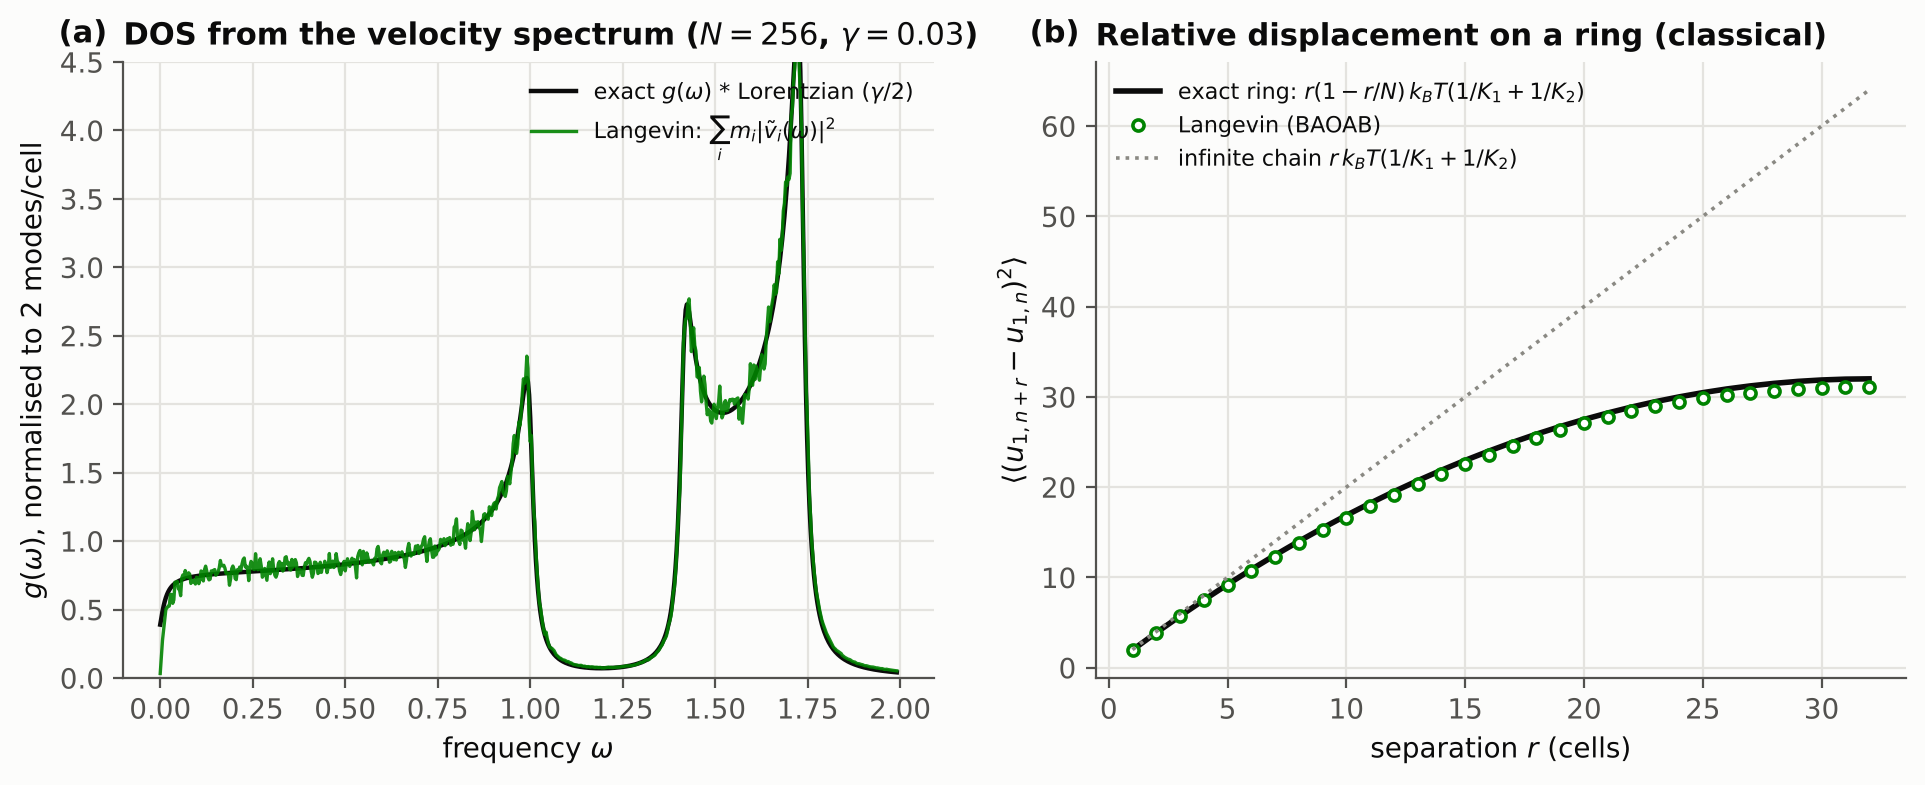
\includegraphics[width=\textwidth]{langevin.png}
\caption{Dinámica de Langevin (BAOAB, $\Delta t=0.05$, $\kB T=1$). (a) Espectro
de velocidades ponderado por masas ($N=256$, $\gamma=0.03$) frente a la DOS
exacta convolucionada con una lorentziana de semianchura $\gamma/2$. (b)
Desplazamiento relativo en un anillo de $64$ celdas ($\gamma=0.5$) frente a la
predicción exacta del puente browniano y a la recta de la cadena infinita.}
\label{fig:langevin}
\end{figure}

% =====================================================================
\section{Implementación numérica}

\subsection{Estructura del código}

\begin{center}
\small
\begin{tabularx}{\textwidth}{@{}l X@{}}
\toprule
Módulo & Contenido\\
\midrule
\code{parameters.py} & \code{ChainParameters}: \code{dataclass} inmutable con $m_1,m_2,K_1,K_2,a$ y magnitudes derivadas ($\vs$, gap, $\avg{\omega^2}$, \dots).\\
\code{dispersion.py} & $D(k)$, ramas cerradas (forma de Vieta), autovectores, cociente de amplitudes, velocidad de grupo, malla de Born–von Kármán.\\
\code{real\_space.py} & Matrices $M$ y $K$ de un anillo o cadena abierta y solución de $\det(K-\omega^2M)=0$ (\code{scipy.linalg.eigh}).\\
\code{dos.py} & DOS cerrada, $N(\omega)$ cerrada, histogramas (malla en $k$ y espacio real), DOS ensanchada, DOS de Debye.\\
\code{thermodynamics.py} & Funciones de un oscilador estables numéricamente (\code{expm1}), cuadratura de Gauss–Legendre en $k$, $U,C_V,F,S$, descomposición por ramas, asintóticas.\\
\code{models.py} & Función de Debye 1D, modelos de Debye, Einstein e híbrido, frecuencias características, ajustes, $\Theta_D(T)$.\\
\code{observables.py} & $G_{ss'}(r)$ con cuadratura compuesta, $\avg{u_s^2}$ en anillos finitos, fluctuaciones de enlace.\\
\code{langevin.py} & Integrador BAOAB, simulación completa con estimadores y predicciones exactas para el anillo.\\
\code{plotting.py} & Estilo común de las figuras.\\
\bottomrule
\end{tabularx}
\end{center}

\subsection{Sutilezas numéricas}

\begin{itemize}
\item \textbf{Cancelaciones.} $\omega_-^2$ se calcula como $\det D/\omega_+^2$ y
  $s(\omega)$ en la forma desarrollada; ambas fórmulas evitan restas de números
  casi iguales y mantienen precisión relativa de máquina cuando $k\to0$ u
  $\omega\to0$. Los autovectores de \code{eigh} se combinan con los autovalores
  cerrados por la misma razón.
\item \textbf{Integración en $k$ y no en $\omega$.} El integrando en $k$ es
  analítico; en $\omega$ tiene singularidades $(\omega_c-\omega)^{-1/2}$.
\item \textbf{Bajas temperaturas.} La malla de Gauss–Legendre se parte en
  $k_c=40\kB T/\hbar\vs$. La pendiente $C_V/T$ a $\kB T=10^{-4}$ coincide con la
  teórica en $7$ cifras.
\item \textbf{Integrandos oscilantes.} $G(r)$ contiene $\ee^{\ii kra}$; se usa una
  cuadratura compuesta con un número de paneles que crece con $r$ (coste lineal
  en $r$, en vez del coste cúbico de una regla de Gauss–Legendre de orden alto).
\item \textbf{Reproducibilidad.} El ruido de Langevin usa
  \code{numpy.random.Generator} con semilla fija; todos los números de este
  documento salen de \code{scripts/make\_figures.py}, que los guarda en
  \code{results/results.json}.
\end{itemize}

\subsection{Pruebas}

\code{tests/test\_physics.py} contiene 26 pruebas que comparan el código con
resultados \emph{independientes}: fórmula cerrada frente a diagonalización,
espacio real frente a Bloch, regla de suma acústica, límite monoatómico, traza
y segundo momento, normalización y derivada de $N(\omega)$, límites de $C_V$,
DOS frente a cuadratura en $k$ frente a anillo finito, consistencia
termodinámica, límites de la función de Debye, $\Theta_D(\infty)$, paseo
aleatorio clásico exacto, crecimiento logarítmico a $T=0$, equipartición y
conservación de la energía en Verlet. Se ejecutan con \code{pytest} o con
\code{python tests/run\_tests.py}.

% =====================================================================
\section{Discusión y conclusiones}

\begin{enumerate}
\item \textbf{De lo general a lo particular.} La simetría de traslación
  discreta del \Eesc{} convierte un problema de $2N$ grados de libertad
  acoplados en $N$ problemas $2\times2$; la aproximación armónica convierte el
  cristal en un sistema ideal de osciladores, y la colectividad canónica hace
  que toda la termodinámica dependa solo de $g(\omega)$. La cadena diatómica es
  el ejemplo mínimo en que aparecen todos los ingredientes de un cristal real:
  ramas acústicas y ópticas, gap, singularidades de van Hove y una DOS que no
  es ni de Debye ni de Einstein.
\item \textbf{Ramas.} La rama acústica es la manifestación dinámica de la
  invariancia traslacional (regla de suma); la óptica existe porque hay más de
  un átomo por celda, y el gap porque esos átomos no son equivalentes (masa o
  rigidez distintas).
\item \textbf{Calor específico.} Debye es exacto a bajas temperaturas (solo
  importa $\vs$) y Einstein con $\omega_E^2=\avg{\omega^2}$ es exacto en la
  primera corrección a altas temperaturas. Ninguno describe la región
  intermedia, que es donde se lee la DOS real: errores máximos del $11\%$
  (Debye) y del $6\%$ (híbrido) para $m_2/m_1=2$.
\item \textbf{Modelos y cociente de masas.} Debye se degrada rápidamente con el
  contraste de masas ($37\%$ para $m_2/m_1=20$) porque la escala óptica no la
  fija la velocidad del sonido. El híbrido mejora mucho ese caso, pero conserva
  un error irreducible de $\sim14\%$, el de Debye sobre una rama acústica
  sinusoidal. La temperatura de Debye efectiva varía entre $0.78$ y $1.83$
  veces su valor a $T=0$ según el contraste: una sola $\Theta_D$ no caracteriza
  un sólido con base.
\item \textbf{Fluctuaciones.} En 1D no hay orden posicional de largo alcance:
  $G(r)\propto r$ a $T>0$ y $\propto\ln r$ a $T=0$, en analogía con la
  ausencia de transición de fase en el Ising 1D. Las fluctuaciones locales
  (enlaces) son finitas y muestran el paso del régimen cuántico (punto cero) al
  clásico (equipartición).
\item \textbf{Validación.} Una simulación de Langevin, que no usa modos
  normales, reproduce la DOS (espectro de velocidades), Dulong–Petit (por
  fluctuaciones de energía) y las correlaciones de desplazamiento. Ilustra
  además que un cristal armónico aislado no es ergódico: el equilibrio requiere
  el baño (o la anarmonicidad).
\end{enumerate}

\paragraph{Extensiones naturales.} Cadenas con $p>2$ átomos por celda,
interacciones a segundos vecinos, defectos e impurezas (modos localizados
dentro del gap, detectables con la razón de participación inversa ya
implementada), anarmonicidad (dilatación térmica, conductividad térmica,
problema FPUT) y el paso a 2D y 3D, donde la DOS de Debye deja de ser plana y
aparece la ley $T^3$.

% =====================================================================
\appendix
\section{Derivación de la velocidad del sonido}

Desarrollando $\omega_-^2=\det D/\omega_+^2$ para $k\to0$:
$\det D\simeq K_1K_2a^2k^2/(m_1m_2)$ y $\omega_+^2\simeq\sigma/\mu$, luego
\[
\omega_-^2\simeq\frac{K_1K_2\,\mu}{\sigma\,m_1m_2}\,a^2k^2
=\frac{K_1K_2}{(K_1+K_2)(m_1+m_2)}\,a^2k^2 .
\]

\section{Segundo momento de la DOS}

Como $\operatorname{tr}D(k)=\sigma/m_1+\sigma/m_2=\sigma/\mu$ para todo $k$,
\[
\avg{\omega^2}=\frac{1}{2N}\sum_{k}\left(\omega_-^2+\omega_+^2\right)
=\frac{1}{2N}\sum_k\operatorname{tr}D(k)=\frac{\sigma}{2\mu}.
\]
Para la cadena de referencia, $\avg{\omega^2}=1.5$ y $\sqrt{\avg{\omega^2}}=1.2247$.

\section{Desplazamiento relativo clásico}

En la cadena infinita, el hamiltoniano en función de los momentos y de los
estiramientos $\epsilon_j$ de cada enlace es una suma de términos cuadráticos
independientes, de modo que $\avg{\epsilon_j^2}=\kB T/K_j$ y
$\avg{\epsilon_j\epsilon_l}=0$ para $j\neq l$. La diferencia
$u_{1,n+r}-u_{1,n}$ es la suma de $r$ enlaces $K_1$ y $r$ enlaces $K_2$, luego
$G_{11}(r)=r\kB T(1/K_1+1/K_2)$. En un anillo, la restricción
$\sum_j\epsilon_j=0$ convierte el paseo en un puente browniano y aparece el
factor $(1-r/N)$.

\section{Reproducibilidad}

\begin{verbatim}
git clone https://github.com/jesus-garcia-izquierdo/diatomic-chain
cd diatomic-chain
pip install -r requirements.txt
python tests/run_tests.py          # 26 pruebas
python scripts/make_figures.py     # figuras + results/results.json
\end{verbatim}

% =====================================================================
\begin{thebibliography}{9}
\bibitem{garcia} P.~García González, \emph{Termodinámica y Física Estadística II},
  apuntes del Grado en Física, Universidad Autónoma de Madrid (2024--2025).
\bibitem{uam} \emph{Mecánica Estadística}, apuntes de máster (temas 1--4),
  Universidad Autónoma de Madrid.
\bibitem{mec} \emph{Mecánica clásica y cuántica: los cinco elementos de un
  problema físico}, notas de curso.
\bibitem{am} N.~W.~Ashcroft y N.~D.~Mermin, \emph{Solid State Physics},
  Saunders (1976), caps.~22--23.
\bibitem{kittel} C.~Kittel, \emph{Introduction to Solid State Physics}, 8.ª ed.,
  Wiley (2005), caps.~4--5.
\bibitem{pathria} R.~K.~Pathria y P.~D.~Beale, \emph{Statistical Mechanics},
  3.ª ed., Elsevier (2011), cap.~7.
\bibitem{lm} B.~Leimkuhler y C.~Matthews, «Rational construction of stochastic
  numerical methods for molecular sampling», \emph{Appl.\ Math.\ Res.\ Express}
  \textbf{2013}, 34--56.
\bibitem{peierls} R.~Peierls, \emph{Quantum Theory of Solids}, Oxford (1955).
\end{thebibliography}

\end{document}
